\documentclass[parskip=full]{scrartcl} % enables german formatting

\usepackage[utf8]{inputenc} % use utf8 file encoding for TeX sources
\usepackage[T1]{fontenc} % avoid garbled Unicode text in pdf
\usepackage[german]{babel} % german hyphenation, quotes, etc
\usepackage{hyperref} % detailed hyperlink/pdf configuration
\usepackage{setspace} % to set spacings between lines
\usepackage{parskip}
\usepackage{graphicx}
\hypersetup{ % ‘texdoc hyperref‘ for options
pdftitle={PSE},
bookmarks=true,
}
\usepackage{csquotes} % provides \enquote{} macro for "quotes"

\usepackage[section]{placeins} % Bilder sollen nicht in andere Kapitel ragen

% Abbildungen mit Kapiteln numerieren
\usepackage{chngcntr}
\counterwithin{figure}{section}

\title{Konfigurator für OSM-Datenaufbereitungs-Prozesse für die Verkehrsnachfragemodellierung}
\subtitle{Pflichtenheft}


\author{Felix Weik\\ Jan-Philipp Hansen\\ Karl Bernhard\\ Pascal Dawideit\\ Simon Schupp}
\date{Dezember 2022}



\begin{document}




\maketitle
\newpage

\tableofcontents
\newpage




\section{Zielbestimmung}
Ob mit dem Fahrrad zur Uni oder mit dem Auto zum Supermarkt: Verkehr betrifft uns alle. Dieses Produkt generiert aus Geodaten des freien Projektes 'Open Street Map' (OSM) eine numerische Wertung der Attraktivität geografischer Standorte. Ein Hauptaugenmerk liegt hierbei auf der Konfigurierbarkeit der Generierung dieser Wertung. Verkehrsplaner können so die richtigen Daten für ihre Verkehrsnachfragemodelle einfach generieren.

\subsection{Musskriterien}
Musskriterien (kurz MK): unabdingbare Leistungen der Software.

\begin{itemize}
    \item <MK1> Der Nutzer muss Projekte erstellen, laden und verwalten können.
    \item <MK2> Der Nutzer muss OSM-Datensätze einlesen können.
    \item <MK3> Der Nutzer muss Kartenausschnitte auswählen können.
    \item <MK4> Der Nutzer muss OSM-Elemente mithilfe von Black- und Whitelisten zu Kategorien zusammenfassen und verwalten können.
    \item <MK5> Das Programm muss Standard-Kategorien anbieten.
    \item <MK6> Das Programm muss OSM-Elemente auf einen Punkt reduzieren können.
    \item <MK7> Das Programm muss den OSM-Elementen Attribute zuweisen können.
    \item <MK8> Der Nutzer muss für jede Kategorie das Verfahren zur Berechnung der Attribute auswählen können.
    \item <MK9> Der Nutzer muss Standardwerte für Attribute festlegen können.
    \item <MK10> Der Nutzer muss Attraktivitätsattribute je Kategorie in Abhängigkeit zu Attributen definieren können.
    \item <MK11> Das Programm muss in jeder Verkehrszelle die Attraktivitätsattribute aggregieren können.
    \item <MK12> Das Programm muss die Zwischenschritte der Berechnungen und Konfigurationen speichern und laden können.
    \item <MK13> Der Nutzer muss die Berechnungen aus jeder Phase aus starten können.
    \item <MK14> Es muss eine grafische Oberfläche geben.
    \item <MK15> Der Nutzer muss Einstellungen des Programms ändern können.
\end{itemize}


\subsection{Wunschkriterien}
Wunschkriterien (kurz WK): wünschenswerte Leistungen der Software.
\begin{itemize}
    \item <WK1> Der Nutzer kann OSM-Daten per Link oder OSM-Repository einlesen..
    \item <WK2> Der Nutzer kann zum Filtern der Kategorien beliebige aussagenlogische Formeln angeben.
    \item <WK3> Das Programm bietet eine Liste an OSM-Key Vorschlägen an.
    \item <WK4> Das Programm kann die Ergebnisse der Aggregation grafisch darstellen.
    \item <WK5> Die Anwendung markiert Phasen, falls sie vom Nutzer abgeändert werden.
    \item <WK6> Die Anwendung besitzt eine Statusanzeige, die den aktuellen Fortschritt der Berechnungen anzeigt.
    \item <WK7> Der Nutzer kann die Attraktivitätsattribute auch in Abhängigkeit zu OSM-Tags definieren.
    \item <WK8> Der Nutzer kann Kategorien von der Berechnung ausschließen.
    
\end{itemize}

\subsection{Abgrenzungskriterien}
Abgrenzungskriterien (kurz AK): Leistungen, die von der Software nicht erbracht werden.
\begin{itemize}
    \item <AK1> Es findet keine Analyse der generierten Daten statt.
    \item <AK2> Die Anwendung ist nicht für Mobilgeräte optimiert.
    \item <AK3> Es findet keine Analyse der Straßennetze statt.
\end{itemize}
\newpage

\section{Produkteinsatz}

\subsection{Anwendungsbereiche}
Dieses Kapitel erläutert, in welchen Bereichen das Produkt eingesetzt werden kann. Die größte Anwendung findet das Produkt bei der Nutzung von Verkehrsnachfragemodellen. Diese benötigen eine Bewertung von Verkehrszellen nach ihrer Attraktivität, um aussagekräftige Vorhersagen treffen zu können. Auf Grundlage dieser Vorhersagen können dann verkehrsplanerische, sowie politische Entscheidungen getroffen werden.


\subsection{Zielgruppen}
Dieser Abschnitt definiert die Zielgruppe des Projekts. Prinzipiell kann jede Person die Anwendung nutzen. Nutzer müssen jedoch Grundkenntnisse im OSM-Dateiformat besitzen. Daher bilden Verkehrsingenieure und Verkehrswissenschaftler die größte Zielgruppe des Produkts. Da die Zielgruppe insbesondere nicht aus Informatikern besteht, werden keine Kenntnisse in der Programmierung vorausgesetzt.
\newpage

\section{Produktübersicht}
In diesem Kapitel werden die Produktfunktionen beschrieben und in einem Use-Case-Diagramm visualisiert. Das Use-Case-Diagramm zeigt mittels Verbindungslinien, wie die einzelnen Use-Cases zueinander stehen. Der Abschnitt „Pipeline-Schritte“ wird genauer in einem Aktivitätsdiagramm abgebildet. Dadurch können die einzelnen Schritte, die durchlaufen werden, besser beschrieben werden.

\subsection*{Abbildung 3.1}
In dem Use-Case-Diagramm „Aufbau der Anwendung“ sieht man die allgemeine Struktur der Anwendung. Der Nutzer befindet sich zu Beginn im Main Menu und kann von dort aus zwischen verschiedenen Möglichkeiten wählen.
Zunächst kann der Nutzer ein neues Projekt erstellen und diesem einen Namen zuweisen. Außerdem ist es möglich, ein zuvor abgespeichertes Projekt zu laden. Von dort aus kann der Nutzer dann die einzelnen Schritte der Anwendung durchlaufen und berechnen lassen. 
Zusätzlich kann der Nutzer die Optionen öffnen und dort Speicherort, Name und Beschreibung des Projektes ändern.

\subsection*{Abbildung 3.2}
Im Aktivitätsdiagramm „Pipeline“ durchläuft der Nutzer alle Schritte des Konfigurators für OSM-Datenaufbereitungs-Prozesse. Dabei kann dieser zunächst auswählen, ob ein neues Projekt erstellt oder ein bestehendes Projekt geladen werden soll. Danach wird der OSM-Datensatz, sowie die shape-Dateien der Verkehrszellen, eingelesen und die Konfiguration der Kategorien optional geladen. Anschließend legt der Nutzer die Kategorien fest und erstellt dafür die Black- und Whitelist. Als nächstes wird für die Reduktion die Berechnungsmethode festgelegt und für die Tags werden Default-Werte eingetragen. Danach gibt der Nutzer für die Kategorien eine Berechnungsmethode an, welche sich aus Tags und Faktoren zusammensetzt. Zuletzt bestimmt der Nutzer noch die Aggregationsmethode innerhalb der Verkehrszellen. Nachdem die Anwendung die Berechnung zu Ende ausgeführt hat, kann der Nutzer das Ergebnis, sowie die Konfiguration exportieren. 
\begin{figure}
    \centering
    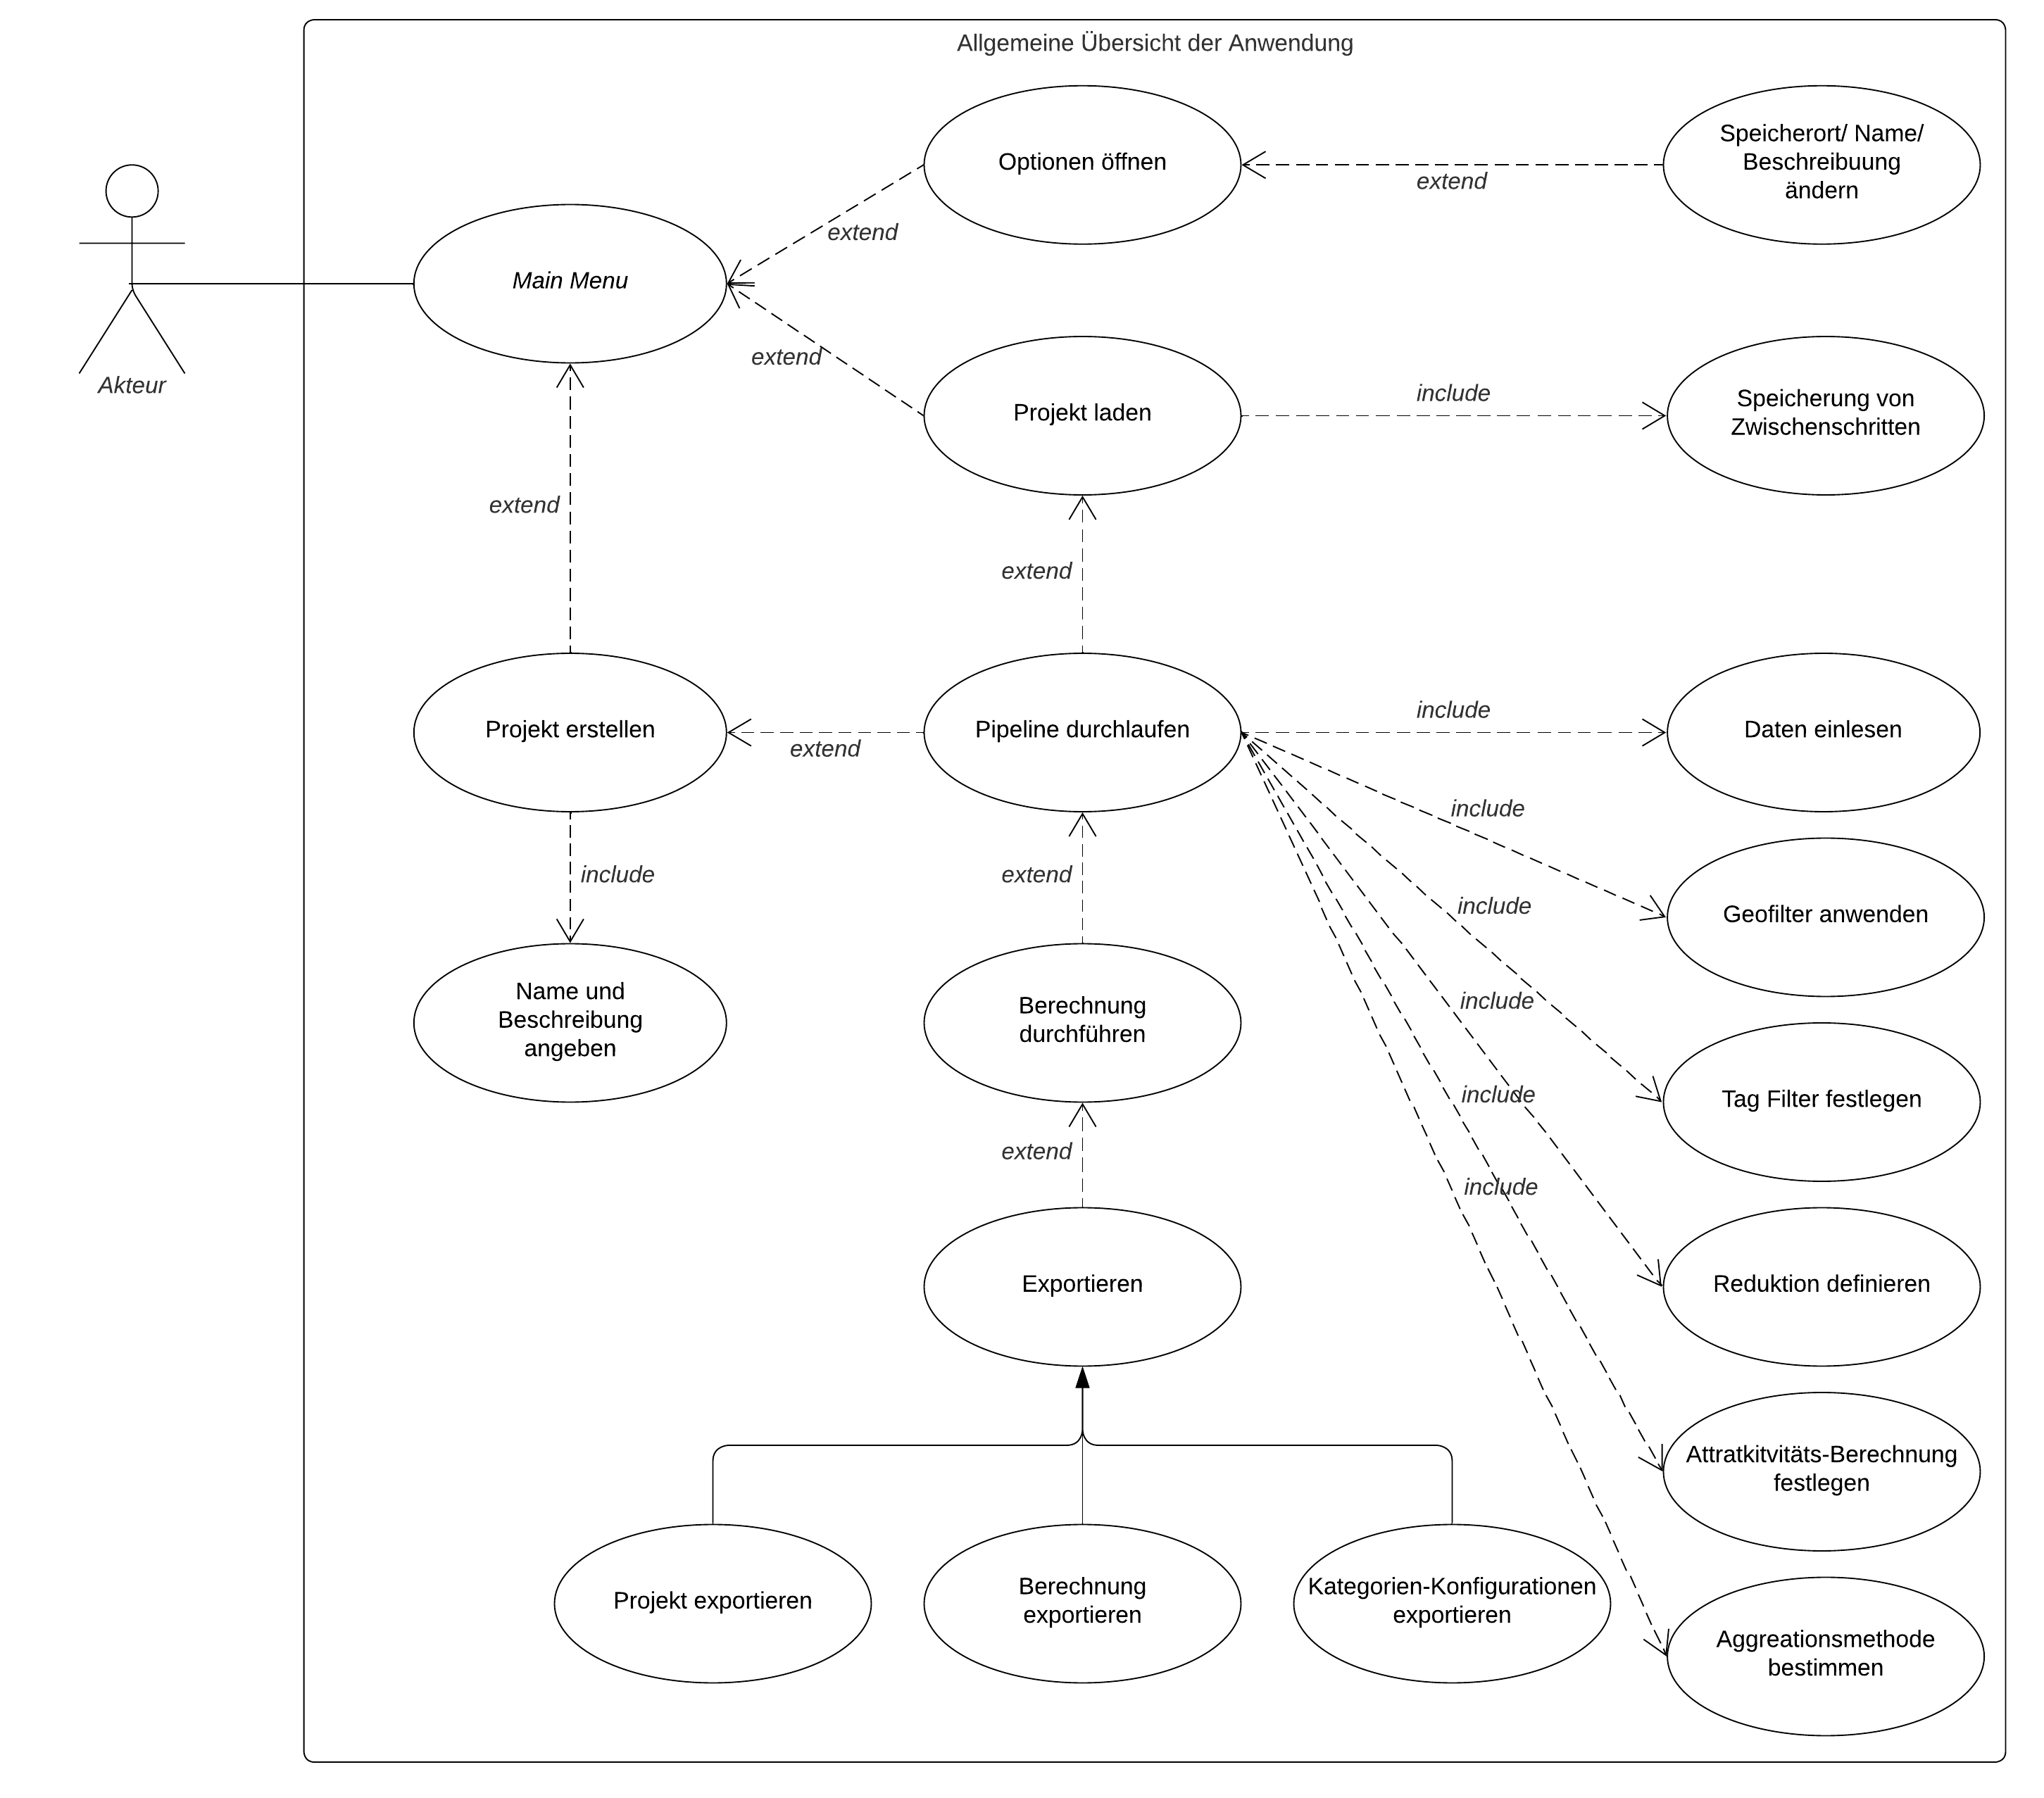
\includegraphics[width=1\textwidth]{pictures/Anwendungsfalldiagramm.png}
    \caption{Use-Case-Diagramm}
\end{figure}

\begin{figure}
    \centering
    \includegraphics[width=.9\textwidth]{pictures/Aktivitätsdiagramm.png}
    \caption{Aktivitätsdiagramm - Durchlaufen der Pipeline}
\end{figure}


\section{Produktfunktionen}
In diesem Kapitel werden die Produktfunktionen erläutert. Wir unterscheiden hier zwischen Funktionen, die die Konfiguration betreffen und Funktionen, die die Berechnungen betreffen. Die Funktionen der Konfiguration sind im ersten Unterkapitel als Katalog von Anwendungsfällen dargestellt. Im zweiten Kapitel ist ein größeres Testszenario angegeben. Die Funktionen der Berechnung werden im dritten Unterkapitel beschrieben.

\subsection{Anwendungsfälle}
Dieser Abschnitt definiert die Funktionen des Produkts mittels konkreter Anwendungsfälle. Für jeden Anwendungsfall werden die funktionalen Anforderungen aufgelistet, die dieser umsetzt. In der Testphase können Tester diesen Katalog nutzen um die korrekte Umsetzung der jeweiligen Produktfunktionen zu überprüfen. Dazu ist für jeden Anwendungsfall eine Vorbedingung, Nachbedingungen, das auslösende Ereignis und eine genaue Beschreibung angegeben. Alternativen und Erweiterungen der Anwendungsfälle konkretisieren die mögliche Umsetzung von Wunschkriterien.
\newpage


\subsubsection*{Starten des Programms <A1>}
\textbf{Anwendungsfall:}  Der Nutzer möchte das Programm starten.\\\\
\textbf{Ziel:} Das Starten des Programms. \\\\
\textbf{Vorbedingung:} Das Programm muss installiert sein.  \\\\
\textbf{Nachbedingung Erfolg:} Das Programm läuft erfolgreich, das Hauptmenü wird angezeigt.\\\\
\textbf{Nachbedingung Fehlschlag:} Das Programm startet nicht. \\\\
\textbf{Auslösendes Ereignis:} Der Nutzer startet das Programm. \\\\
\textbf{Beschreibung:}
\begin{enumerate}
    \item Das Hauptmenü wird angezeigt.
\end{enumerate}
\newpage


\subsubsection*{Neues Projekt erstellen <A2>}
\textbf{Anwendungsfall:} Der Nutzer möchte ein neues Projekt erstellen.\\\\
\textbf{Anforderungen:} MK1\\\\
\textbf{Ziel:} Erstellen eines neuen Projekts. \\\\
\textbf{Vorbedingung:} Der Nutzer befindet sich im Hauptmenü. \\\\
\textbf{Nachbedingung Erfolg:} Ein neues Projekt befindet sich im Speicher. Die Seite 'Data' ist geöffnet.  \\\\
\textbf{Nachbedingung Fehlschlag:} Die Anwendung informiert den Nutzer über den Fehlschlag. Der Nutzer befindet sich im Hauptmenü. \\\\
\textbf{Auslösendes Ereignis:} Der Nutzer drückt, den erstelle ein neues Projekt Knopf. \\\\
\textbf{Beschreibung:}
\begin{enumerate}
    \item Der Nutzer wählt den Namen und die Beschreibung für das Projekt.
    \item Der Nutzer wählt den Speicherort des Projekts aus.
    \item Der Nutzer drückt, auf den erstelle neues Projekt Knopf.
    \item Das Projekt wird erstellt und der Projektordner am angegebenen Speicherort angelegt.
\end{enumerate}
\newpage


\subsubsection*{Internes Projekt laden <A3>}
\textbf{Anwendungsfall:} Der Nutzer möchte ein Projekt aus dem Projektstandardordner laden.\\\\
\textbf{Anforderungen:} MK1 \\\\
\textbf{Ziel:} Das Laden eines Projektes aus dem Projektstandardordner. \\\\
\textbf{Vorbedingung:} Der Nutzer befindet sich im Hauptmenü.  \\\\
\textbf{Nachbedingung Erfolg:} Alle Daten des Projekts sind geladen und die Seite 'Data' wird angezeigt. \\\\
\textbf{Nachbedingung Fehlschlag:} Benachrichtigung des Nutzers über Fehlschlag, Programm  bleibt im Hauptmenü. \\\\
\textbf{Auslösendes Ereignis:}  Der Nutzer wählt ein Projekt aus und drückt den "lade ausgewähltes Projekt" Knopf. \\\\
\textbf{Beschreibung:}
\begin{enumerate}
    \item Das ausgewählte Projekt wird geladen.
    \item Die Anwendung zeigt die Seite 'Data' an.
\end{enumerate}
\newpage


\subsubsection*{Externes Projekt laden <A4>}
\textbf{Anwendungsfall:} Der Nutzer möchte ein Projekt außerhalb des Projektstandardordners laden.\\\\
\textbf{Anforderungen:} MK1\\\\
\textbf{Ziel:} Ein Projekt wird geladen. \\\\
\textbf{Vorbedingung:} Der Nutzer befindet sich im Hauptmenü.  \\\\
\textbf{Nachbedingung Erfolg:} Alle Daten des Projekts sind geladen und die Seite 'Data' wird angezeigt. \\\\
\textbf{Nachbedingung Fehlschlag:} Benachrichtigung des Nutzers über Fehlschlag, der Nutzer bleibt im Hauptmenü. \\\\
\textbf{Auslösendes Ereignis:}  Der Nutzer drückt den 'lade externes Projekt' Knopf. \\\\
\textbf{Beschreibung:}
\begin{enumerate}
    \item Der Datei-Explorer öffnet sich.
    \item Der Nutzer wählt einen Projektordner aus.
    \item Die Anwendung lädt das ausgewählte Projekt.
    \item Die Anwendung zeigt die Seite 'Daten' an.
\end{enumerate}
\newpage



\subsubsection*{Einstellungen ändern im Hauptmenü <A5>}
\textbf{Anwendungsfall:} Der Nutzer möchte Änderungen der Einstellungen des Programms vornehmen. \\\\
\textbf{Anforderungen:} MK15\\\\
\textbf{Ziel:} Einstellungen des Programms ändern.\\\\
\textbf{Vorbedingung:}  Der Nutzer befindet sich im Hauptmenü.  \\\\
\textbf{Nachbedingung Erfolg:} Die Änderung der Einstellungen werden angezeigt.\\\\
\textbf{Nachbedingung Fehlschlag:} Die Anwendung informiert den Nutzer über den Fehlschlag.\\\\
\textbf{Auslösendes Ereignis:} Drücken desEinstellungsknopfes Knopfes. \\\\
\textbf{Beschreibung:}
\begin{enumerate}
    \item Die Seite 'Settings' öffnet sich.
    \item Der Nutzer kann den Projektstandardordner versetzen.
    \item Die Anwendung nimmt die Änderungen vor.
\end{enumerate}
\newpage



\subsubsection*{Dateien referenzieren <A6>}
\textbf{Anwendungsfall:} Der Nutzer möchte den Geofilter und die Eingabedateien festlegen.\\\\
\textbf{Anforderungen:} MK2, MK3, WK1 \\\\
\textbf{Ziel:} Der Nutzer definiert die OSM-Daten und den räumlichen Filter.\\\\
\textbf{Vorbedingung:} Der Nutzer befindet sich auf der Seite 'Data'. \\\\
\textbf{Nachbedingung Erfolg:} Erfolgreiches Hinterlegen der angegebenen Dateien. Anzeigen der angegebenen Dateien.\\\\
\textbf{Nachbedingung Fehlschlag:} Benachrichtigung des Nutzers über Fehlschlag. \\\\
\textbf{Auslösendes Ereignis:} Drücken des Knopfes 'Select OSM-Data'.\\\\
\textbf{Beschreibung:}
\begin{enumerate}
    \item Der Datei-Explorer öffnet sich.
    \item Der Nutzer wählt eine {OSM-Datei}~\ref{dataformat} aus.
    \item Die Anwendung zeigt den Namen der gewählten Datei an.
    \item Der Nutzer drückt auf den Knopf 'Select Cut-Out'.
    \item Der Datei-Explorer öffnet sich.
    \item Der Nutzer wählt eine \hyperlink{dataformat}{Datei mit Verkehrszellen} aus.
    \item Die Anwendung zeigt den Namen der gewählten Datei an.
    \item Der Nutzer wählt eine der folgenden Optionen aus.
    \begin{itemize}
        \item Im räumlichen Filter befinden sich nur OSM-Elemente, welche sich vollständig in den angegebenen Verkehrszellen befinden.
        \item Im räumlichen Filter befinden sich auch OSM-Elemente, welche sich nur teilweise in den angegebenen Verkehrszellen befinden.
    \end{itemize}
\end{enumerate}
\textbf{Alternative:}
\begin{itemize}
    \item 2a: Der Nutzer gibt die URL eines OSM-Repository an.
\end{itemize}
\newpage


% Noch nicht fertig, wir müssen noch besprechen, wo das stattfindet
\subsubsection*{Kategorien importieren <A7>}
\textbf{Anwendungsfall:} Der Nutzer möchte in seinem Projekt Kategorien verwenden, welche bereits in einem anderen definiert sind.\\\\
\textbf{Anforderungen:} MK4, MK12\\\\
\textbf{Ziel:} Das Importieren vordefinierter Kategorien. \\\\
\textbf{Vorbedingung:} Der Nutzer befindet sich auf der Seite 'Data'. \\\\
\textbf{Nachbedingung Erfolg:} Die Kategorien der importierten Datei sind in der Liste der Kategorien aufgelistet. \\\\
\textbf{Nachbedingung Fehlschlag:} Die Anwendung informiert den Nutzer über den Fehlschlag. \\\\
\textbf{Auslösendes Ereignis:} Drücken des Knopfes zum Importieren der Kategorien.\\\\
\textbf{Beschreibung:}
\begin{enumerate}
    \item Der Datei-Explorer öffnet sich.
    \item Der Nutzer wählt eine Datei im \hyperlink{dataformat}{passenden Format} aus.
    \item Die Anwendung zeigt den Namen der ausgewählten Datei an.
    \item Der Nutzer bestätigt den Import der Kategorien.
    \item Die Anwendung fügt die Kategorien zur Kategorienliste hinzu.
\end{enumerate}
\textbf{Erweiterungen:} 
\begin{itemize}
    \item 3a: Neben dem Namen der Datei werden auch die in ihr enthaltenen Daten visualisiert.
\end{itemize}
\textbf{Alternativen:} 
\begin{itemize}
    \item 5a: Die Anwendung ersetzt die bisherigen Kategorien mit den importierten.
\end{itemize}
\newpage


\subsubsection*{Erstellen von Kategorien <A8>}
\textbf{Anwendungsfall:} Der Nutzer möchte eine weitere Kategorie hinzufügen.\\\\
\textbf{Anforderungen:} MK4\\\\
\textbf{Ziel:} Die Liste der Kategorien soll um eine weitere Kategorie ergänzt werden. \\\\
\textbf{Vorbedingung:} Der Nutzer befindet sich auf der Seite 'Categories'. \\\\
\textbf{Nachbedingung Erfolg:} In der Liste der Kategorien befindet sich eine neue, nicht-konfigurierte Kategorie. Die neue Kategorie ist ausgewählt.\\\\
\textbf{Auslösendes Ereignis:} Der Nutzer drückt auf den Button zum Hinzufügen einer neuen Kategorie. \\\\
\textbf{Beschreibung:}
\begin{enumerate}
    \item Die Anwendung schreibt einen leeren Eintrag in die Kategorienliste.
    \item Die Anwendung wählt den neuen Eintrag aus.
\end{enumerate}
\newpage


\subsubsection*{Auswählen von Kategorien <A9>}
\textbf{Anwendungsfall:} Der Nutzer möchte eine Kategorie auswählen, um diese genauer zu betrachten.\\\\
\textbf{Anforderungen:} MK5, MK4\\\\
\textbf{Ziel:} Das Auswählen und Anzeigen einer Kategorie. \\\\
\textbf{Vorbedingung:} Der Nutzer befindet sich auf der Seite 'Categories'. Es existiert mindestens eine Kategorie. \\\\
\textbf{Nachbedingung Erfolg:} Name, Whitelist und Blacklist der neuen Kategorie wird angezeigt.\\\\
\textbf{Nachbedingung Fehlschlag:} Die Seite bleibt unverändert.\\\\
\textbf{Auslösendes Ereignis:} Der Nutzer drückt auf das Dropdown-Menü zum Auswählen der Kategorie. \\\\
\textbf{Beschreibung:}
\begin{enumerate}
    \item Die Anwendung zeigt eine Liste aller Kategorien.
    \item Beim ersten Öffnen befinden sich bereits Standardkategorien in der Liste.
    \item Der Nutzer wählt eine der Kategorien aus.
    \item Die Anwendung zeigt den Namen, die Whitelist und die Blacklist der Kategorie an.
\end{enumerate}
\newpage


\subsubsection*{Konfigurieren von Kategorien <A10>}
\textbf{Anwendungsfall:} Der Nutzer möchte die Eigenschaften einer Kategorie verändern.\\\\
\textbf{Anforderungen:} MK4, WK2, WK3, WK8\\\\
\textbf{Ziel:} Konfigurieren einer Kategorie \\\\
\textbf{Vorbedingung:} Der Nutzer befindet sich auf der Seite 'Categories'. Es existiert mindestens eine Kategorie.\\\\
\textbf{Nachbedingung Erfolg:} Die Änderungen an der Kategorie und an ihren Eigenschaften wird angezeigt. \\\\
\textbf{Nachbedingung Fehlschlag:} Die Anwendung zeigt den Grund für den Fehlschlag an. \\\\
\textbf{Auslösendes Ereignis:} Der Nutzer wählt eine Kategorie aus oder erstellt eine neue Kategorie. \\\\
\textbf{Beschreibung:}
\begin{enumerate}
    \item Die Anwendung zeigt dem Nutzer den Namen, die Whitelist und die Blacklist der Kategorie an. Die Anwendung signalisiert, ob die Kategorie aktiviert ist.
    \item Der Nutzer kann keine, eine oder mehrere der folgenden Aktionen durchführen:
    \begin{itemize}
        \item Der Nutzer kann den Namen der Anwendung ändern.
        \item Der Nutzer kann Einträge zur Blacklist und zur Whitelist hinzufügen und entfernen.
    \end{itemize}
\end{enumerate}
\textbf{Erweiterung:}
\begin{itemize}
    \item 1a: Die Anwendung schlägt in einer Liste OSM-Tags vor.
    \item 2a: Der Nutzer kann die Kategorie aktivieren oder deaktivieren. Die Anwendung blendet deaktivierte Kategorien auf den kommenden Seiten aus.
\end{itemize}
\textbf{Alternativen:}
\begin{itemize}
    \item 2b: Statt den Tag-Filter durch eine Whitelist und Blacklist zu definieren, kann der Nutzer einen beliebigen regulären Ausdruck angeben.
\end{itemize}
\newpage


\subsubsection*{Löschen von Kategorien <A11>}
\textbf{Anwendungsfall:} Der Nutzer möchte eine Kategorie löschen.\\\\
\textbf{Anforderungen:} MK4\\\\
\textbf{Ziel:} Das Entfernen einer Kategorie aus der Kategorienliste.\\\\
\textbf{Vorbedingung:} Der Nutzer befindet sich auf der Seite 'Categories'. Es existiert mindestens eine Kategorie. Eine Kategorie ist ausgewählt.\\\\
\textbf{Nachbedingung Erfolg:} Die ausgewählte Kategorie befindet sich nicht mehr in der Liste. Es ist keine Kategorie mehr ausgewählt.\\\\
\textbf{Nachbedingung Fehlschlag:} Die Liste der Kategorien ändert sich nicht.\\\\
\textbf{Auslösendes Ereignis:} Der Nutzer drückt auf den Button zum Löschen einer Kategorie. \\\\
\textbf{Beschreibung:}
\begin{enumerate}
    \item Die Anwendung löscht die Kategorie.
\end{enumerate}
\textbf{Erweiterung:}
\begin{itemize}
    \item 0a: Die Anwendung fordert den Nutzer auf die Löschung zu bestätigen.
\end{itemize}
\newpage


\subsubsection*{Punktreduktion definieren <A12>}
\textbf{Anwendungsfall:} Der Nutzer möchte den Ablauf der Punktreduktion definieren.\\\\
\textbf{Anforderungen:} MK6, MK8\\\\
\textbf{Ziel:} Definition der Punktreduktion. \\\\
\textbf{Vorbedingung:} Der Nutzer befindet sich auf der Seite 'Reduction'.\\\\
\textbf{Nachbedingung Erfolg:} Die geänderten Einstellungen werden angezeigt. \\\\
\textbf{Nachbedingung Fehlschlag:} Die Anwendung informiert den Nutzer über den Fehlschlag. \\\\
\textbf{Auslösendes Ereignis:} Der Nutzer wählt eine Kategorie aus. \\\\
\textbf{Beschreibung:}
\begin{enumerate}
    \item Der Nutzer kann entscheiden, ob für die Berechnung der Attribute ausschließlich Standardwerte benutzt werden sollen.
    \item Der Nutzer kann entscheidet, ob eine Fläche berechnet werden soll.
    \item Falls ja, entscheidet der Nutzer, ob die Fläche des Grundstücks oder des Gebäudes berechnet werden soll.
    \item Der Nutzer entscheidet, ob die Geschossfläche berechnet werden soll.
\end{enumerate}
\newpage


\subsubsection*{Standardwerte für Attribute festlegen <A13>}
\textbf{Anwendungsfall:} Der Nutzer möchte für eine Kategorie und ein Attribut einen Standardwert angeben.\\\\
\textbf{Anforderungen:} MK8, MK9\\\\
\textbf{Ziel:} Festlegen eines Standardwertes eines Attributs für eine Kategorie. \\\\
\textbf{Vorbedingung:} Der Nutzer befindet sich auf der Seite 'Reduction'. \\\\
\textbf{Nachbedingung Erfolg:} Die Standardwerte sind hinterlegt. \\\\
\textbf{Nachbedingung Fehlschlag:} Die Anwendung informiert den Nutzer über den Fehlschlag. \\\\
\textbf{Auslösendes Ereignis:} Der Nutzer wählt eine Kategorie aus. \\\\
\textbf{Beschreibung:}
\begin{enumerate}
    \item Der Nutzer klickt auf den Reiter zum Festlegen der Standardwerte.
    \item Die Anwendung zeigt die Liste der Tags für die Standardwerte an.
    \item Der Nutzer erstellt einen neuen Eintrag in der Tag-Liste oder wählt einen bereits erstellten Eintrag aus.
    \item Die Anwendung zeigt die bisherigen Standardwerte der Attribute für diesen Eintrag an.
    \item Der Nutzer kann den Tag-Listen-Eintrag verändern.
    \item Der Nutzer kann die Reihenfolge der Tag-Listen-Einträge verändern.
    \item Der Nutzer legt je Attribut den Standardwert fest.
\end{enumerate}
\newpage


\subsubsection*{Attraktivitätsattribute konfigurieren <A14>}
\textbf{Anwendungsfall:} Der Nutzer möchte für eine Kategorie Attraktivitätsattribute definieren.\\\\
\textbf{Anforderungen:} MK10, WK7\\\\
\textbf{Ziel:} Konfigurieren der Attraktivitätsattribute. \\\\
\textbf{Vorbedingung:} Der Nutzer befindet sich auf der Seite 'Attractivity'. \\\\
\textbf{Nachbedingung Erfolg:} Die Änderungen an der Konfiguration sind sichtbar. \\\\
\textbf{Nachbedingung Fehlschlag:} Der Nutzer wird über den Fehler informiert. \\\\
\textbf{Auslösendes Ereignis:} Der Nutzer wählt eine Kategorie aus \\\\
\textbf{Beschreibung:}
\begin{enumerate}
    \item Der Nutzer wählt ein Attraktivitätsattribut aus oder erstellt ein neues.
    \item Der Nutzer kann das Attraktivitätsattribut löschen, den Namen ändern und je Attribut einen Faktor festlegen.
\end{enumerate}
\textbf{Erweiterungen:} 
\begin{itemize}
    \item 0a: Der Nutzer kann durch Drücken eines Buttons eine Übersicht aller Berechnungen von allen Attraktivitätsattributen in allen Kategorien öffnen. 
    \item 2a: Der Nutzer kann auch Tags Faktoren zuweisen.
\end{itemize}
\newpage


\subsubsection*{Wählen der Aggregation-Verfahren <A15>}
\textbf{Anwendungsfall:} Der Nutzer möchte unterschiedliches Aggregations-Verfahren wählen.\\\\
\textbf{Anforderungen:} MK11\\\\
\textbf{Ziel:} Es wurde ausgewählt, welche Aggregation-Verfahren berechnet werden sollen.\\\\
\textbf{Vorbedingung:} Der Nutzer befindet sich auf der Seite 'Aggregation'.\\\\
\textbf{Nachbedingung Erfolg:} Es werden die vom Nutzer gewählten Aggregationverfahren angezeigt.\\\\
\textbf{Nachbedingung Fehlschlag:} Die Anwendung zeigt den Grund für den Fehlschlag an. \\\\
\textbf{Auslösendes Ereignis:} Der Nutzer aktiviert oder deaktiviert die Checkbox eines Aggregation-Verfahrens. \\\\
\textbf{Beschreibung:}
\begin{enumerate}
    \item Der Nutzer setzt Hacken in die Checkbox, von den Aggregation-Verfahren, die er berechnen will.
\end{enumerate}
\newpage


\subsubsection*{Berechnungen durchführen <A16>}
\textbf{Anwendungsfall:} Der Nutzer hat das Projekt konfiguriert und möchte nun die Berechnungen starten.\\\\
\textbf{Anforderungen:} MK7, MK11, MK13, WK4, WK5, WK6\\\\
\textbf{Ziel:} Das Durchführen der Berechnungen und das Generieren des Endergebnisses.\\\\
\textbf{Vorbedingung:} Der Nutzer befindet sich auf der Seite 'Calculate'. Alle Konfigurationsphasen sind konfiguriert.\\\\
\textbf{Nachbedingung Erfolg:} Das Endresultat ist berechnet und kann unter 'Export' exportiert werden. \\\\
\textbf{Nachbedingung Fehlschlag:} Die Anwendung informiert den Nutzer über die Berechnungsphase, in welcher der Fehlschlag passiert. \\\\
\textbf{Auslösendes Ereignis:} Der Nutzer wählt eine Berechnungsphase und drückt den Button 'Calculate from selected'.\\\\
\textbf{Beschreibung:}
\begin{enumerate}
    \item Die Anwendung beginnt die Berechnung in der ausgewählten Berechnungsphase. (für Details siehe \hyperlink{calculations}{Berechnungen}).
    \item Die Anwendung zeigt dem Nutzer die aktuelle Berechnungsphase an.
    \item Die Anwendung beendet die Berechnung.
    \item Der Nutzer exportiert die generierten Daten.
\end{enumerate}
\textbf{Erweiterungen:} 
\begin{itemize}
    \item 0a: Die Anwendung informiert den Nutzer über Berechnungsphasen, die neu berechnet, werden müssen.
    \item 2a: Die Anwendung approximiert den prozentualen Fortschritt der Berechnungen.
    \item 2b: Der Nutzer kann die Berechnung pausieren und sie fortsetzen.
    \item 3a: Der Nutzer kann die Daten visualisieren.
\end{itemize}
\newpage



\subsubsection*{Neuberechnung <A17>}
\textbf{Anwendungsfall:}  Der Nutzer möchte die Berechnung neu starten.\\\\
\textbf{Ziel:} Neustarten der Berechnung.\\\\
\textbf{Vorbedingung:} Die Anwendung berechnet gerade oder die Berechnungen sind abgeschlossen. Der Nutzer befindet sich auf der Seite 'Calculate'.\\\\
\textbf{Nachbedingung Erfolg:} Die Berechnungen sind unterbrochen und der Nutzer kann sie neu-starten.\\\\
\textbf{Auslösendes Ereignis:} Der Nutzer drückt den 'Cancel' Knopf während der Berechnung oder den 'Recalculate' Knopf am Ende der Berechnung.\\\\
\textbf{Beschreibung:}
\begin{enumerate}
    \item Die Berechnung wird abgebrochen, sofern sie nicht schon beendet ist.
    \item Die Berechnungs-Seite wird auf die Startposition zurückgesetzt.
\end{enumerate}
\newpage



\subsubsection*{Darstellen der Berechnungsergebnisse <A18>}
\textbf{Anwendungsfall:} Der Nutzer möchte die berechneten Daten visualisieren.\\\\
\textbf{Anforderungen:} WK4\\\\
\textbf{Ziel:} Visualisierung der Daten.\\\\
\textbf{Vorbedingung:}  Der Nutzer befindet sich auf der Seite 'Calculate'.\\\\
\textbf{Nachbedingung Erfolg:} Die Anwendung zeigt ein Diagramm der berechneten Daten an.\\\\
\textbf{Nachbedingung Fehlschlag:} Die Anwendung zeigt den Grund für den Fehlschlag an.\\\\
\textbf{Auslösendes Ereignis:} Der Nutzer drückt den Knopf 'Visualize Results'.\\\\
\textbf{Beschreibung:}
\begin{enumerate}
    \item Die Anwendung zeigt ein Diagramm an, in dem die berechneten Daten visualisiert sind.
\end{enumerate}
\newpage



\subsubsection*{Phase wechseln <A19>}
\textbf{Anwendungsfall:} Der Nutzer möchte in eine andere Phase der Konfigurierung wechseln.\\\\
\textbf{Ziel:} Die aktuelle Konfigurationsseite wird gespeichert und eine andere geladen. \\\\
\textbf{Vorbedingung:} Ein Projekt ist geladen. \\\\
\textbf{Nachbedingung Erfolg:} Die ausgewählte Seite wird angezeigt. Änderungen der alten Seite sind gespeichert.\\\\
\textbf{Nachbedingung Fehlschlag:} Die alte Seite wird weiterhin angezeigt. Die Anwendung informiert den Nutzer über den Fehlschlag. \\\\
\textbf{Auslösendes Ereignis:} Drücken auf eine Phase im Kopf der Seite oder Drücken auf einen 'Continue' Button. \\\\
\textbf{Beschreibung:}
\begin{enumerate}
    \item Die Anwendung speichert die Daten, die der Nutzer auf der aktuellen Seite hinterlegt hat.
    \item Die Anwendung lädt die Daten für die ausgewählte bzw. nächste Seite.
    \item Die Anwendung öffnet die ausgewählte bzw. nächste Seite.
\end{enumerate}
\textbf{Erweiterungen:} 
\begin{itemize}
    \item 3a: Die Anwendung informiert den Nutzer über die Speicherung der Daten.
\end{itemize}
\newpage


\subsubsection*{Exportieren des Endergebnisses <A20>}
\textbf{Anwendungsfall:} Der Nutzer möchte das Endergebnis exportieren.\\\\
\textbf{Anforderungen:} MK12\\\\
\textbf{Ziel:} Exportieren des Endergebnisses an einen gewünschten Speicherplatz\\\\
\textbf{Vorbedingung:}  Der Nutzer befindet sich innerhalb eines Projekts.\\\\
\textbf{Nachbedingung Erfolg:} An der vom Nutzer definierten Stelle befindet sich ein ZIP-Archiv, welches das Endergebnis enthält. \\\\
\textbf{Nachbedingung Fehlschlag:} Die Anwendung zeigt den Grund für den Fehlschlag an.\\\\
\textbf{Auslösendes Ereignis:} Der Nutzer drückt den Button 'Export' \\\\
\textbf{Beschreibung:}
\begin{enumerate}
    \item Der Nutzer drückt auf 'Calculations Export'
    \item Der Datei-Explorer öffnet sich.
    \item Der Nutzer wählt einen Speicherort aus.
    \item Die Anwendung komprimiert das Endergebnis zu einem ZIP-Archiv und speichert es an angegebener Stelle ab.
\end{enumerate}
\newpage



\subsubsection*{Exportieren des Projektes <A21>}
\textbf{Anwendungsfall:} Der Nutzer möchte das Projekt exportieren. \\\\
\textbf{Anforderungen:} MK12\\\\
\textbf{Ziel:} Das Exportieren des Projektes an einen Speicherort.\\\\
\textbf{Vorbedingung:} Der Nutzer befindet sich innerhalb eines Projekts.\\\\
\textbf{Nachbedingung Erfolg:} Ein ZIP-Archiv mit dem Projekt befindet sich an der vom Nutzer angegebenen Stelle.\\\\
\textbf{Nachbedingung Fehlschlag:} Die Anwendung informiert den Nutzer über den Fehlschlag.\\\\
\textbf{Auslösendes Ereignis:}  Der Nutzer drückt unter 'Export' auf den Button 'Project Export' \\\\
\textbf{Beschreibung:}
\begin{enumerate}
    \item Der Datei-Explorer öffnet sich.
    \item Der Nutzer wählt den passenden Speicherort aus.
    \item Der Nutzer bestätigt das Exportieren des Projektes.
    \item Die Anwendung exportiert das Projekt.
\end{enumerate}
\newpage




\subsubsection*{Exportieren der Konfigurationen <A22>}
\textbf{Anwendungsfall:} Der Nutzer möchte die Kategorien des Projektes exportieren.\\\\
\textbf{Anforderungen:} MK1, MK12\\\\
\textbf{Ziel:} Die Konfiguration der Kategorien befindet sich an der vom Nutzer angegebenen Stelle.\\\\
\textbf{Vorbedingung:} Der Nutzer befindet sich innerhalb eines Projekts.\\\\
\textbf{Nachbedingung Erfolg:} Die Konfigurationsdatei befindet sich an der vom Nutzer angegebenen Stelle\\\\
\textbf{Nachbedingung Fehlschlag:}  Die Anwendung informiert den Nutzer über den Fehlschlag.\\\\
\textbf{Auslösendes Ereignis:} Der Nutzer drückt unter 'Export' auf 'Configuration Export' \\\\
\textbf{Beschreibung:}
\begin{enumerate}
    \item Der Datei-Explorer öffnet sich.
    \item Der Nutzer wählt den passenden Speicherort aus.
    \item Der Nutzer bestätigt das Exportieren der Kategorien.
    \item Die Anwendung exportiert die Konfiguration.
\end{enumerate}
\newpage



\subsubsection*{Einstellungen vornehmen <A23>}
\textbf{Anwendungsfall:} Der Nutzer möchte die Einstellungen verändern.\\\\
\textbf{Anforderungen:} MK1, MK15\\\\
\textbf{Ziel:} Ändern der allgemeinen Einstellungen des Projekts und der Anwendung. \\\\
\textbf{Vorbedingung:} Der Nutzer befindet sich in einem Projekt oder im Hauptmenü.\\\\
\textbf{Nachbedingung Erfolg:} Der Nutzer befindet sich auf der Seite 'Settings'. Die Änderungen an den Einstellungen sind vorgenommen. \\\\
\textbf{Nachbedingung Fehlschlag:} Die Anwendung informiert den Nutzer über den Fehlschlag. \\\\
\textbf{Auslösendes Ereignis:} Der Nutzer drückt auf den Knopf zum Öffnen der Einstellungen. \\\\
\textbf{Beschreibung:}
\begin{enumerate}
    \item Befindet sich der Nutzer in einem Projekt, so kann er den Namen und die Beschreibung von diesem ändern.
    \item Der Nutzer kann den Projektstandardordner setzen.
\end{enumerate}
\newpage


\subsubsection*{Anwendung beenden <A24>}
\textbf{Anwendungsfall:} Der Nutzer möchte die Anwendung schließen.\\\\
\textbf{Ziel:} Die Anwendung soll sich schließen und nicht-gespeicherte Daten speichern. \\\\
\textbf{Vorbedingung:} Die Anwendung ist gestartet.\\\\
\textbf{Nachbedingung Erfolg:} Die Anwendung ist geschlossen und nicht-gespeicherte Daten sind gespeichert.\\\\
\textbf{Nachbedingung Fehlschlag:} Die Anwendung ist noch geöffnet.\\\\
\textbf{Auslösendes Ereignis:} Drücken auf das Kreuz, zum Beenden der Anwendung, welches durch das Betriebssystem üblich ist. \\\\
\textbf{Beschreibung:}
\begin{enumerate}
    \item Befindet sich der Nutzer auf einer Konfigurationsseite mit nicht-gespeicherten Daten, so werden diese zwischengespeichert.
    \item Die Anwendung schließt sich.
\end{enumerate}
\textbf{Erweiterungen:} 
\begin{itemize}
    \item 1a: Gibt es nicht-gespeicherte Daten, so wird der Nutzer aufgefordert diese zu speichern oder zu verwerfen.
\end{itemize}
\newpage





\subsection{Testszenario}
\subsubsection*{Transfer von Kategorien <S1>}
\textbf{Anwendungsfall:} Nutzer $A$ hat ein Projekt $P_A$ erstellt und in diesem Kategorien definiert. Nutzer $B$ möchte dieselben Kategorien in einem anderen Projekt $P_B$ verwenden.\\\\
\textbf{Ziel:} Transfer der Kategorien von $P_A$ nach $P_B$.\\\\
\textbf{Vorbedingung:} Nutzer $A$ hat ein Projekt konfiguriert.\\\\
\textbf{Nachbedingung Erfolg:} Die Kategorien von Nutzer $A$ befinden sich im Projekt von Nutzer $B$.\\\\
\textbf{Beschreibung:}
\begin{enumerate}
    \item Nutzer $A$ startet die Anwendung und lädt das Projekt $P_A$.
    \item Nutzer $A$ klickt auf 'Export' und dann 'Configurations Export'.
    \item Die Anwendung öffnet den Datei-Explorer.
    \item Nutzer $A$ wählt einen Speicherort der Konfigurations-Datei $D$ aus.
    \item Nutzer $A$ sendet $D$ per E-Mail an $B$.
    \item Nutzer $B$ startet die Anwendung und lädt das Projekt $P_B$.
    \item Nutzer $B$ drückt unter 'Data' den Button zum Importieren von Kategorien.
    \item Die Anwendung öffnet den Datei-Explorer
    \item Nutzer $B$ wählt die Datei $D$ aus.
    \item Der Nutzer bestätigt den Import.
    \item Die Anwendung lädt die Kategorien in Projekt $P_B$.
\end{enumerate}
\newpage






\subsection{Berechnungsablauf} \hypertarget{calculations}{}
Dieser Abschnitt beschreibt den Ablauf der Berechnungsphasen. Es gibt folgende Berechnungsphasen:
\begin{enumerate}
    \item Dateninput und Geofilter,
    \item Tag Filter,
    \item Reduktion,
    \item Attraktivität,
    \item Aggregation.
\end{enumerate}
Die Abarbeitung der Berechnungsphasen kann in jeder Phase gestartet werden, läuft die Phasen aber dann in der gegebenen Reihenfolge durch.

\subsubsection*{Dateninput und Geofilter}
\begin{itemize}
    \item Die Anwendung liest die in A6 referenzierte OSM-Datei D1 ein.
    \item Die Anwendung liest die in A6 definierte Verkehrszellen-Datei D2 ein.
    \item Die Anwendung generiert eine neue OSM-Datei D3. In dieser befinden sich die OSM-Elemente aus D1, die sich in den Verkehrszellen aus D2 befinden. Die Einordnung von Elementen, die sich nicht vollständig in den Verkehrszellen befinden, ist in A6 definiert.
\end{itemize}


\subsubsection*{Tag Filter}
\begin{itemize}
    \item Die Anwendung weist den OSM-Elementen aus D3 Kategorien zu. Ein OSM-Element befindet sich in einer Kategorie, wenn
    \begin{itemize}
        \item es alle Tag-Einträge der Whitelist der Kategorie (A10) erfüllt \textbf{und}
        \item es keinen Tag-Eintrag der Blacklist der Kategorie (A10) erfüllt.
        \item alternativ (WK2): es dem in angegebenen regulären Ausdruck (A10.2b) entspricht.
    \end{itemize}
    \item Die Ergebnisse werden in einer Datei D4 gespeichert.
\end{itemize}


\subsubsection*{Reduktion}
\begin{itemize}
    \item Die Anwendung projiziert je Kategorie alle OSM-Elemente (aus D4) jeweils auf eine Koordinate.
    \item Die Anwendung weißt jedem OSM-Elemente in jeder Kategorie den Attributen (wie in A12 konfiguriert) Werte zu.
    \item Kann oder soll die Anwendung einem Attribut keinen Wert zuweisen, so weißt sie ihm einen Standardwert zu. Dazu wird der tiefste Tag-Listen-Eintrag (wie in A13 konfiguriert) gewählt, den das OSM-Element erfüllt.
    \item Die Anwendung speichert je Kategorie und OSM-Element die generierten Koordinaten und Attribute in einer Datei D5.
\end{itemize}


\subsubsection*{Attraktivität}
\begin{itemize}
    \item Die Anwendung berechnet in jeder Kategorie für jedes (in A14) konfigurierte Attraktivitätsattribut. Sei $X$ die Menge der Attribute, $v(x)$ der Wert des Attributes $x$ und $f(x)$ der (in A14) definierte Faktor des Attributs zu einem festen Attraktivitätsattribut $a$. Dann berechnet die Anwendung den Wert $v(a)$ des Attraktivitätsattributs mit der Formel $$v(a)=\sum_{x\in X}{v(x)\cdot f(x)}.$$
    \item Erweiterung (WK7): $X$ enthält neben allen Attributen auch Tags.
    \item Die Anwendung speichert die generierten Attraktivitätsattribute in einer Datei D6.
\end{itemize}

\subsubsection*{Aggregation}
\begin{itemize}
    \item Die Anwendung bestimmt für jedes OSM-Element (in jeder Kategorie) in welchen Verkehrszellen es sich befindet.
    \item Für jede Verkehrszelle aggregiert die Anwendung die Attraktivitätsattribute nach (in A15 aktivierten) Aggregationsverfahren.
    \item Die Anwendung speichert das Endergebnis in der \hyperlink{finalresult}{Ausgabe}.
\end{itemize}
\newpage





\section{Produktdaten} \hypertarget{data}{}
Dieses Kapitel beschreibt die Organisation der Produktdaten. Daten, welche nicht unbedingt erhoben werden müssen, sind mit einem Stern ($\ast$) markiert. Die größte Organisationseinheit sind hierbei die Projekte. Jedem Projekt ist ein Verzeichnis zugeordnet. Dieses Verzeichnis wird im folgenden auch als Projektordner bezeichnet. In jedem Projektordner befinden sich die folgenden Dateien und Verzeichnisse:
\begin{itemize}
    \item Projekt-Konfiguration (JSON-Datei)
    \item Kategorien-Konfiguration (JSON-Datei)
    \item Zwischenergebnisse (Verzeichnis)
    \item Ausgabe (Verzeichnis)
\end{itemize}

\subsection*{Projekt-Konfiguration}
Diese JSON-Datei enthält die wichtigsten Grundeinstellungen des jeweiligen Projektes. Darunter:
\begin{itemize}
    \item Name des Projekts
    \item Beschreibung des Projekts ($\ast$)
    \item Erstellungsdatum des Produkts ($\ast$)
    \item Datum der letzten Änderung ($\ast$)
    \item Definition des räumlichen Filters: Müssen OSM-Elemente vollständig im definierten Bereich liegen, um betrachtet zu werden?
    \item Liste der Statistiken, die während der Aggregation berechnet werden sollen
    \item Verweis auf die OSM-Eingabedatei
    \item Verweis auf die Datei, welche die Verkehrszellen definiert
\end{itemize}


\subsection*{Kategorien-Konfiguration}
Diese JSON-Datei enthält alle Informationen zu den Kategorien des jeweiligen Projekts. Es folgt eine Liste der Eigenschaften, die je Kategorie gespeichert werden müssen.
\begin{itemize}
    \item Name der Datei (eindeutig)
    \item Einträge der Tag-Whitelist
    \item Einträge der Tag-Blacklist
    \item Definition der Default-Werte je Attribut
    \item Konfiguration der Punktreduktion
    \item Faktoren der Attribute je Attraktivitätsattribut
\end{itemize}


\subsection*{Zwischenergebnisse}
Dieses Verzeichnis enthält die Zwischenergebnisse der Berechnungen der jeweiligen Phasen.

\subsection*{Ausgabe} \hypertarget{finalresult}{}
Dieses Verzeichnis enthält die finale Ausgabe der Berechnungen. Hier befindet sich je ausgewähltem Aggregationsverfahren eine CSV-Datei. Jede dieser CSV-Dateien ordnet jeder Verkehrszelle je Attraktivitätsattribut einen numerischen Wert zu.


\subsection*{Anwendungsdaten}
Neben den projektspezifischen Daten gibt es auch Daten, die für die ganze Anwendung Relevanz haben. Diese sind:
\begin{itemize}
    \item Der Nutzer kann Projekte bzw. ihre Projektordner grundsätzlich an beliebigen Stellen speichern. Jedoch gibt es einen Projektstandardordner. In diesem werden Projekte standardmäßig gespeichert. Die GUI ermöglicht ein nutzerfreundlicheres Öffnen von Projekten aus dem Projektstandardordner. Der Nutzer kann den Projektstandardordner beliebig versetzen.
    \item Es gibt eine Liste von Tags, die dem Nutzer vorgeschlagen werden. Diese muss verwaltet werden.
\end{itemize}


\subsection*{Dateiformate} \hypertarget{dataformat}{}
Zum Lesen der anwendungsspezifischen Daten verwendet die Anwendung Dateiformate:
\begin{itemize}
    \item OSM-Dateien: Zum Lesen und Speichern von OSM-Elementen unterstützt die Anwendung die Dateiformate .osm.bz2 und .osm.pbz.
    \item Verkehrszellen: Zum Definieren von Verkehrszellen verwendet die Anwendung die Dateiformate shape und geojson.
\end{itemize}


\newpage







\section{Nichtfunktionale Anforderungen}

Dieses Kapitel definiert die nichtfunktionalen Anforderungen und Qualitätsmerkmale der Software.

Reminder: Punktreduktion soll erweiterbar sein



\subsection{Funktionalität}

\begin{tabular}{|l| c| c| c| c|}
    \hline
        Produktqualität & sehr gut & gut & normal & nicht relevant \\
    \hline
        Angemessenheit & & x & &\\
    \hline
        Richtigkeit & x & & &\\
    \hline
        Ordnungsmäßgkeit & x & & &\\
    \hline
        Interoperabilität & & & & x\\
    \hline
        
    \end{tabular}

\textbf{Angemessenheit}
\newline
Die Angemessenheit ist als gut einzustufen, da die gesamte Software für ihre Funktion geeignet sein muss und eine schwere Handhabung der Software nur zu unnötigem Aufwand seitens des Nutzers führt.



\textbf{Richtigkeit und Ordnungsmäßigkeit}
\newline
Die Aufgabe der Software ist über die Konfigurationen des Nutzers und den eingelesenen Dateien, neue Daten zu berechnen, welche weiter verwendet werden können. Hierbei ist es wichtig, dass diese Daten auch korrekt berechnet werden und ein deterministisches Verhalten gewährleistet ist.
Daher ist die Richtigkeit und Ordnungsmäßigkeit der Software als sehr gut einzustufen.

\textbf{Interoperabilität}
\newline
Es ist keine Kommunikation zwischen Geräten vorgesehen, daher ist die Interoperabilität als irrelevant einzustufen.


% remove this if we dont want to have a new page for each
% subsection
\newpage 

\subsection{Sicherheit}

    \begin{tabular}{|l| c| c| c| c|}
    \hline
        Produktqualität & sehr gut & gut & normal & nicht relevant \\
    \hline
        Zuverlässigkeit & x & & &\\
    \hline
        Fehlertoleranz & & x & &\\
    \hline
        Wiederherstellbarkeit & & x & &\\
    \hline
     \end{tabular}

\textbf{Zuverlässigkeit\\}
Die Zuverlässigkeit ist wichtig, da Benutzer erwarten, dass die Anwendung konsistente Ergebnisse liefert.
Es wird erwartet, dass das Programm die eingegebenen Daten basierend auf Benutzereingaben korrekt auswertet.
Durch das Definieren von Testfällen in dem Pflichtenheft und das Ausführen dieser Testfälle während der Implementierungsphase können Fehler frühzeitig erkannt und behoben werden.
Dies gewährleistet eine sehr gute Zuverlässigkeit.

\textbf{Fehlertoleranz\\}
Trotz aller Testfälle, kann es zu Fehlern kommen, während das Programm läuft. Diese Fehler können entstehen durch korrumpierte Daten oder durch fehlerhafte Eingabe des Users.
Fehler die durch falsche Eingabe des Users entstehen können abgefangen werden und der User benachrichtigt werden, somit kann dieser die fehlerhafte Eingabe korrigieren.
Fehler die ausgelöst werden durch korrumpierte Daten, können behoben werden indem der User benachrichtigt wird und dieser die korrumpierte Daten ersetzt.
Da diese Fehler nur entstehen können durch das falsche Verhalten des Users, kann 
die Fehlertoleranz als gut eingestuft werden.

\textbf{Wiederherstellbarkeit\\}
Beim Erstellen der Konfigurationen kann der Nutzer zu jedem Zeitpunkt die Konfigurationen lokal zwischenspeichern. Diese kann er zu einem späteren Zeitpunkt wieder einlesen. Dadurch wird gewährleistet, dass die Konfigurationsentscheidungen des Nutzers einfach wiederhergestellt werden können.
Auch alle Zwischenergebnisse, der vom Programm durchgeführten Berechnungen, werden direkt nach Fertigstellung auf dem Endgerät gespeichert. Während der einzelnen Berechnungen sind jedoch keine Zwischenspeicherungen vorgesehen.
Somit ist die Wiederherstellbarkeit als gut einzustufen.


% remove this if we dont want to have a new page for each
% subsection
\newpage 


\subsection{Benutzbarkeit, author = Felix}

    \begin{tabular}{|l| c| c| c| c|}
    \hline
        Produktqualität & sehr gut & gut & normal & nicht relevant \\
    \hline
        Verständlichkeit & x & & &\\
    \hline
        Erlernbarkeit & & x & &\\
    \hline
        Bedienbarkeit & x & & &\\
    \hline
        Effizienz & & & x &\\
    \hline
        Zeitverhalten & & & x &\\
    \hline
        Verbrauchsverhalten & & x & &\\
    \hline
    \end{tabular}

\textbf{Verständlichkeit, Erlernbarkeit und Bedienbarkeit}\\
Die Anwendung soll intuitiv zugänglich sein, um ein reibungsloses Einlesen der Daten zu ermöglichen. Da die Anwendung auch an Nicht-Informatiker gerichtet ist, muss die Bedienung leicht einsehbar und verständlich sein. Dies erfolgt über eine moderne GUI.

\textbf{Effizienz, Zeitverhalten und Verbrauchsverhalten}\\
Die Effizienz der Anwendung ist als normal eingestuft, da kein schnelles Reaktionsverhalten in der Berechnung gefordert ist, trotzdem aber eine gewisse Benutzerfreundlichkeit erhalten bleiben werden muss. Folglich soll die Anwendung ein gutes Zeit- und Verbrauchsverhalten haben.
Eine kleine Instanz (bspw. Stadtkreis Karlsruhe) ist auf einem Laptop mit 8GB RAM innerhalb weniger Stunden berechenbar. Für größere Instanzen wird eine Workstation empfohlen.


% remove this if we dont want to have a new page for each
% subsection
\newpage 


\subsection{Änderbarkeit}
    \begin{tabular}{|l| c| c| c| c|}
    \hline
        Produktqualität & sehr gut & gut & normal & nicht relevant \\
    \hline
        Analysierbarkeit & x & & & \\
    \hline
        Modifizierbarkeit & x & & &\\
    \hline
        Stabilität & x & & &\\
    \hline
        Prüfbarkeit & & & x &\\
    \hline
        Übertragbarkeit & & & x &\\
    \hline
        Anpassbarkeit & x & & &\\
    \hline
        Installierbarkeit & & & x &\\
    \hline
    \end{tabular}
    
\textbf{Analysierbarkeit, Modifizierbarkeit und Anpassbarkeit}\\
Erweiterungen stellen ein häufig gewünschtes Kriterium dar. Deshalb ist das Produkt gut modifizierbar. Um Änderungen und Erweiterungen, wie das Hinzufügen von Verfahren bei der Reduktion oder Methoden bei der Aggregation, umzusetzen ist jedoch Code-Verständnis erforderlich und diese müssen von einem Informatiker implementiert werden. Die Anpassbarkeit des Produktes ist gut. Änderungen an der Benutzeroberfläche beziehungsweise der Implementierung der Berechnungs-Verfahren beeinflussen sich nicht untereinander. Um dies zu gewährleisten, muss der Programmcode übersichtlich, strukturiert, kommentiert und somit sehr gut analysierbar sein.

\textbf{Stabilität}\\
Die Benutzeroberfläche darf die Funktionalität des Produktes nicht beeinträchtigen. Daher muss eine gute Stabilität gewährleistet werden.

\textbf{Installierbarkeit}\\
Das Produkt ist als Open-Source-Anwendung online erhältlich als .exe-Datei. Die Installierbarkeit ist als normal einzustufen.


% remove this if we dont want to have a new page for each
% subsection
\newpage 


\subsection{Qualitätsanforderungen}
In diesem Abschnitt werden die oben genannten Qualitätseigenschaften als konkrete Qualitätsanforderungen formuliert.

\begin{itemize}
    \item <Q1> Die Anwendung soll in englischer Sprache verfügbar sein
    \item <Q2> Die Anwendung soll intuitiv bedienbar sein
    \item <Q3> Die Anwendung muss auf Windows 10 und 11 nutzbar sein
    \item <Q4> Durch eine 80-prozentige Testabdeckung soll die Korrektheit des Produkts gewährleistet sein
    \item <Q5> Das Produkt soll um neue Verfahren erweiterbar sein
    \item <Q6> Das Produkt muss als Open-Source-Projekt weiterentwickelbar sein
    \item <Q7> Der Quelltext soll lesbar und kommentiert sein
    \item <Q8> Die Berechnungszeiten sollen minimal sein
    \item <Q9> Die Programmiersprache muss Python sein.
    \item <Q10> Der Programmablauf soll deterministisch sein
    \item <Q11> Die Anwendung soll von unerfahrenen Nutzern leicht installierbar sein
\end{itemize}

\newpage



\section{Benutzeroberfläche/Schnittstellen}
In diesem Kapitel wird die Benutzeroberfläche erläutert. Es wird auf die Darstellung der einzelnen Funktionen sowie die Navigation zwischen diesen eingegangen.

\textbf{Benutzeroberfläche}
Die Anwendung ist für Desktop-Computer konzipiert. Folglich stellt die Benutzeroberfläche einen wichtigen Teil des Produktes dar.
Die Steuerung erfolgt durch Maus- und Tastatureingaben. Das Anwendungsdesign ist in den verschiedenen Navigationskomponenten möglichst einheitlich gestaltet. Für den Nutzer soll die Anwendung intuitiv verständlich sein. Die Übersichtlichkeit spielt eine große Rolle, gleichzeitig soll das Design anregend zur Verwendung sein.
Die Navigation beginnt auf dem Hauptmenü, über das mithilfe von Buttons die weiteren Funktionen aufgerufen werden können.
Innerhalb der folgenden Seiten wird der aktuelle Schritt sowie die Navigation über eine Toolbar am oberen Rand der Anwendung visualisiert. 
Eine entsprechende Visualisierung des Programmworkflows wird in Abbildung 7.3 erläutert.

\textbf{Main Menu }<UI10>
Das Hauptmenü bietet eine erste Übersicht zum Starten des Workflows. Über drei Buttons kann der Workflow durch Laden eines bereits vorhandenen Projekts oder Erstellen eines neuen gestartet werden. Weiter befindet sich rechts der Buttons eine Schaltfläche, die die vergangenen Projekte auflistet und eine Möglichkeit zum Laden bietet. Über einen letzten Knopf lassen sich die Anwendungseinstellungen aufrufen.

\textbf{New Project }<UI20>
Hat der Nutzer im Hauptmenü die Option zum Erstellen eines neuen Projektes aufgerufen, wird er in dieses Fenster geleitet.
Hier besteht die Möglichkeit über Texteingabefelder den Namen sowie die Beschreibung eines neuen Projektes einzugeben. Weiter kann über einen Button der Explorer zum Auswählen eines Speicherortes für das Projekt festgelegt werden. Wird kein Speicherort angegeben, wird ein Projektstandardordner gewählt.
Über zwei Buttons am unteren rechten Rand kann die Projekterstellung bestätigt und begonnen oder abgebrochen werden.

\textbf{Data }<UI30>
Hier können die zur Berechnung wichtigen Daten ausgewählt werden.
Über drei Buttons können die OSM-Daten, der Cutout zur Bereichseingrenzung sowie ein Kopieraufruf gewählt werden. Über eine Checkbox kann angegeben werden, ob Gebäude am Cutout-Rand in die Berechnung miteinbezogen werden sollen.
Entstehen beim Kopieren über "Copy in Configurations" Konflikte bei der Auswahl, gibt das Programm eine Fehlermmeldung aus und fragt den Nutzer nach Bestätigung zum Überschreiben und Mergen (siehe Abbildung 7.17 und 7.18). Hier kann der Nutzer entweder das Überschreiben starten, oder über einen Abbrechen-Button zurück zum Data-Fenster gelangen.

\newpage

\textbf{Categories }<UI40>
Über dieses Fenster kann der Nutzer neue Kategorien erstellen sowie sich bereits erstellte Kategorien anzeigen lassen. Weiter kann er den Kategorien White- und Blacklist Tags zuordnen, die bei der späteren Berechnung miteinbezogen werden.
Über ein Dropdown-Menü können Kategorien ausgewählt werden. In einem enstprechenden Textfeld wird daraufhin der Namen der gewählten Kategorie angezeigt. Eine Liste schlägt Key-Recommendations vor. Weiter können in zwei Tabellen besagte Black- und Whitelist Tags gewählt werden.
Über zwei Buttons am unteren rechten Anwendungsrand können neue Kategorien erstellt oder exitierende gelöscht werden. 
Wird der "Delete" Button gewählt, wird über ein Popup (Abbildung 7.19) nach Bestätigung gefragt. Wurde eine neue Kategorie erstellt, wird diese direkt im DropDown-Menü ausgewählt.

\textbf{Reduction }<UI50>
In diesem Fenster kann der Nutzer festlegen, wie die Flächenberechnung der Kategorien durchgeführt wird. Das Fenster wird dazu in eine linke und rechte Hälfte unterteilt.
Links befindet sich die Liste aller Kategorien, rechts kann der Nutzer deren Reduktion konfigurieren.
Durch das Anklicken einer Kategorie in der Liste links wird rechts eine Schaltfläche angezeigt. Dieses hat 2 Knöpfe: Zum einen den Calculation Knopf. Wird dieser Knopf gedrückt kann festgelegt werden, welche Werte für diese Kategorie berechnet werden sollen, dies geschieht über Checkboxen. Es muss zuerst angegeben werden, ob die Fläche überhaupt berechnet werden soll. Nur wenn diese Option aktiviert ist, werden die Spezifikationen darunter angezeigt. Über einen Schalter kann zwischen der Grundstücks- und Gebäudeflächenberechnung unterschieden werden. Weiter kann gewählt werden, ob diese Fläche mit den Stockwerken multipliziert werden soll oder nicht. Zuletzt kann gewählt werden, ob nur die angegebenen Default-Werte verwendet werden sollen.
Drückt man den "Default-Values" Knopf, so können für Tags Defaultwerte gesetzt werden. Es kann über den "New Tag" Button neue Tags hinzugefügt werden und über den "Delete Tag" Button gelöscht werden. Das Löschen muss in einem Pop-up-Fenster bestätigt werden (Abbildung 7.19).
Jede Kategorie besitzt unlöschbare Default-Werte. Treffen keine Tags zu werden diese zur Berechnung verwendet.
Wann welcher Defaultwert benutzt wird, hängt von der Reihenfolge in der Liste ab, so gilt je weiter oben, desto geringer die Priorität. Über die Pfeilknöpfe an den Tags in der Liste können diese in dieser Prioritätsliste verschoben werden. Es kann dabei nichts über den DEFAULT wert gehen.

\newpage

\textbf{Attractivity }<UI60>
Dieses Fenster beinhaltet zwei Dropdown-Listen. Die obere Liste ist zum Auswählen einer Kategorie, die untere dient der Unterscheidung der jeweiligen Attraktivitäts-Attribute.
Ist eine Kategorie und ein Attraktivitätsattribut ausgewählt, so wird das Namensfeld des Attraktivitätsattributes, die Tag-Factor-List und die Attribut-Faktoren angezeigt.
In der Tag-Factor-List können nun, ähnlich zu den Black- und White-Listen, Tags geschrieben werden. Zu diesen Tags schreibt man einen Faktor dazu.
Bei den Attribute-Factors gibt es drei Standardattribute zur Kategorie. Diese können mit einem Faktor und einer Standard-Attraktivität versehen werden.
Die Buttons "New Attractivity" und "Delete Attractivity" erstellen und löschen Attraktivitätsattribute. Das Löschen muss in einem Pop-up-Fenster bestätigt werden (Abbildung 7.19).
Der Knopf View Attractivity-List zeigt eine Liste an. Dort werden alle Kategorien und deren Attraktivitätsattributen, so wie deren Berechnung angezeigt.
Die Liste ist so aufgebaut, dass ganz links die Kategorie steht, in der Mitte das Attraktivitätsattribut und rechts die zugehörige Berechnung.
Die Liste dient nur der Veranschaulichung und Übersicht. Hier kann nicht editiert werden.
Mit dem Button "Edit Attractivity" kehrt man zum vorherigen Fenster zurück.

\textbf{Aggregation }<UI60>
Im Aggregationsfenster kann festgelegt werden, welche Werte in den Verkehrszellen berechnet werden sollen. Hierzu wird eine Liste mit allen möglichen Berechnungsarten angezeigt. In dieser Liste kann über Checkboxen festgelegt werden, welche Berechnungsarten in der Berechnung getätigt werden sollen.

\textbf{Calculate }<UI70>
Hier wird als letzter Schritt nach fertiger Dateneingabe die Berechnung gestartet. Über eine Schaltfläche am linken Anwendungsrand kann der gewünschte Startpunkt der Berechnung angegeben werden. Hier können beliebig viele Phasen übersprungen werden, ab der die folgenden Schritte in angezeigter Reihenfolge ausgeführt werden. Über den "Start Calculation" Button wird die Berechnung gesartet.
Während der Berechnung informiert ein Ladebalken über den aktuellen Berechnungsstatus. Weiter zeigt die Schaltfläche links die aktuelle Phase als auch die bereits bearbeiteten Phasen an. Über einen Button kann die Berechnung jederzeit abgebrochen werden. Diese Aktion muss über ein Pop-up-Fenster bestätigt werden (Abbildung 7.20).
Nach Vollendung der Berechnung können die Ergebnisse angesehen, oder die Berechnung erneut gestartet werden. Diese Aktion muss über ein Pop-up-Fenster bestätigt werden (Abbildung 7.21).
Die Anwendung informiert den Nutzer über einen Schriftzug, wenn die Berechnung vollendet wurde.

\textbf{Export }<UI80>
Der Export-Knopf im Head Menü öffnet ein Dropdown-Menü mit Buttons für Exportmöglichkeiten. Wird einer der Buttons betätigt, öffnet sich der Explorer zur Speicherortsauswahl.
Durch erneutes Drücken des Export-Knopfs verschwindet das Dropdown-Menü wieder.

\newpage

\textbf{Settings }<UI90>
Im Settings-Fenster der Anwendung können Einstellungen zum aktuellen Projekt vorgenommen werden.
Die Einstellungen gliedern sich in zwei Teile.
Im ersten Teil können Daten zum Projekt geändert werden. Über eine Schaltfläche können im Nachhinein Projektname und die zugehörige Beschreibung angepasst werden. Wurde das Settings-Fenster ohne ein offenes Projekt geöffnet, wird dieser Teil nicht angezeigt.
Im zweiten Teil können Einstellungen zur Anwendung vorgenommen werden. Hier kann der Nutzer über einen Button den Standardordner zur Projektspeicherung festlegen.
Alle Änderungen können über zwei Buttons entweder gespeichert oder verworfen werden.

\newpage

\begin{figure}
    \centering
    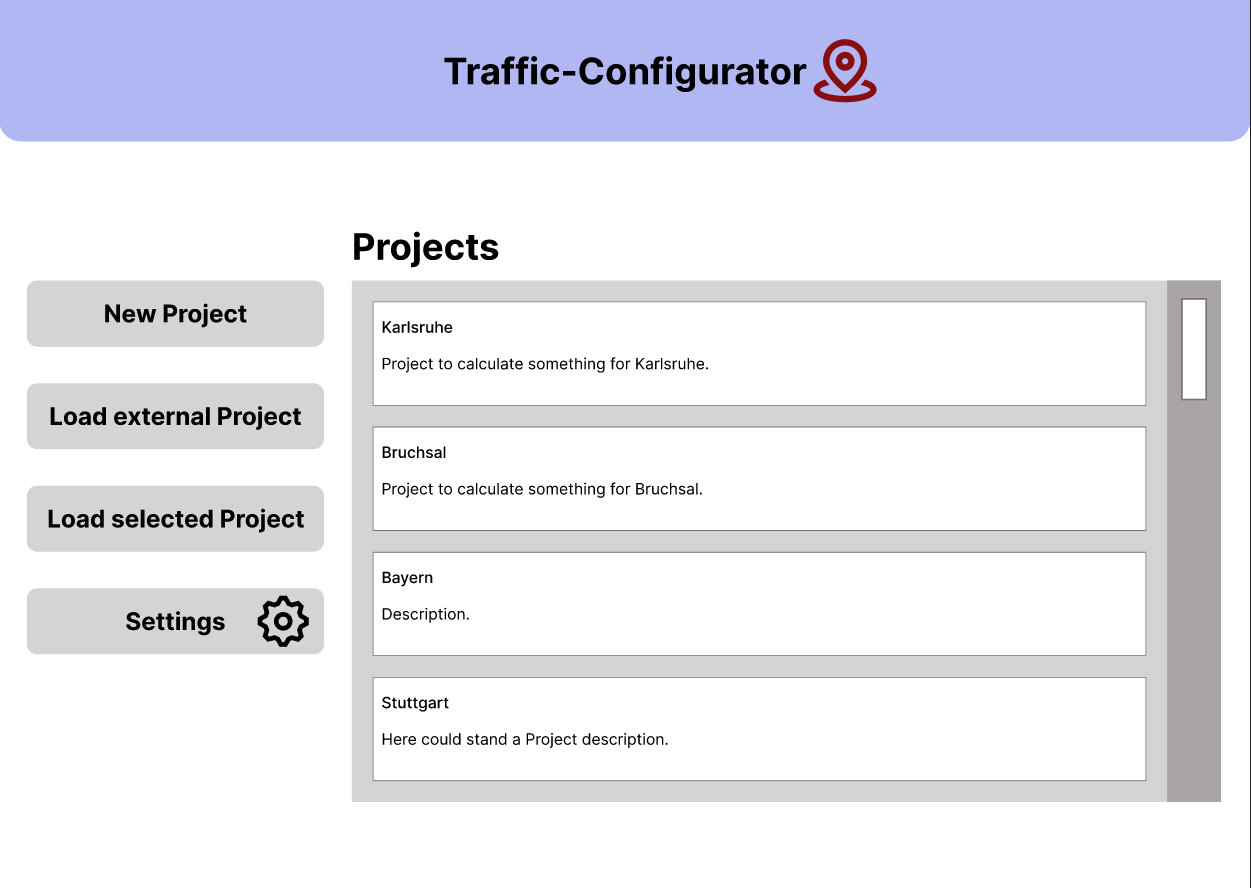
\includegraphics[width=1\textwidth]{pictures/Main Menu.png}
    \caption{Main Menu}
\end{figure}

\begin{figure}
    \centering
    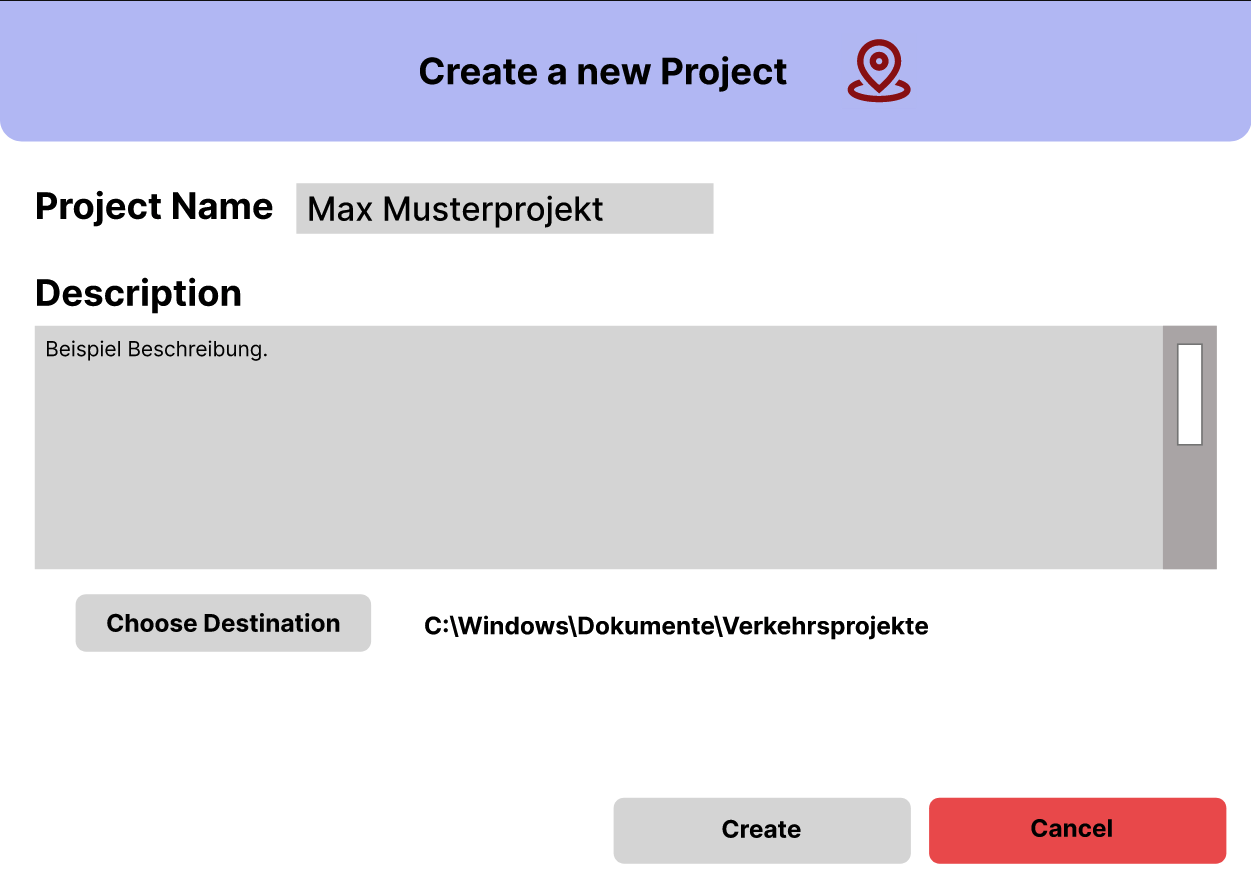
\includegraphics[width=1\textwidth]{pictures/New Project.png}
    \caption{New Project}
\end{figure}

%Grafik zur Workflowvisualisierung
\begin{figure}
    \centering
    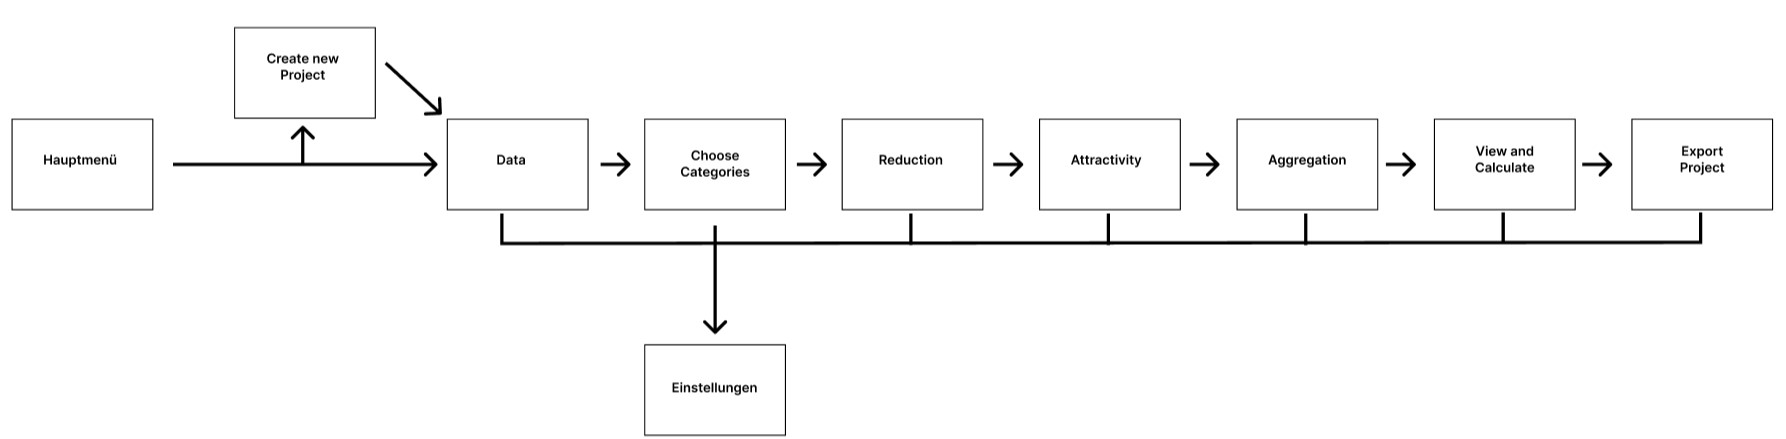
\includegraphics[width=1\textwidth]{pictures/WorkflowvisualisierungGUI.jpg}
    \caption{Workflowvisualisierung}
\end{figure}

\begin{figure}
    \centering
    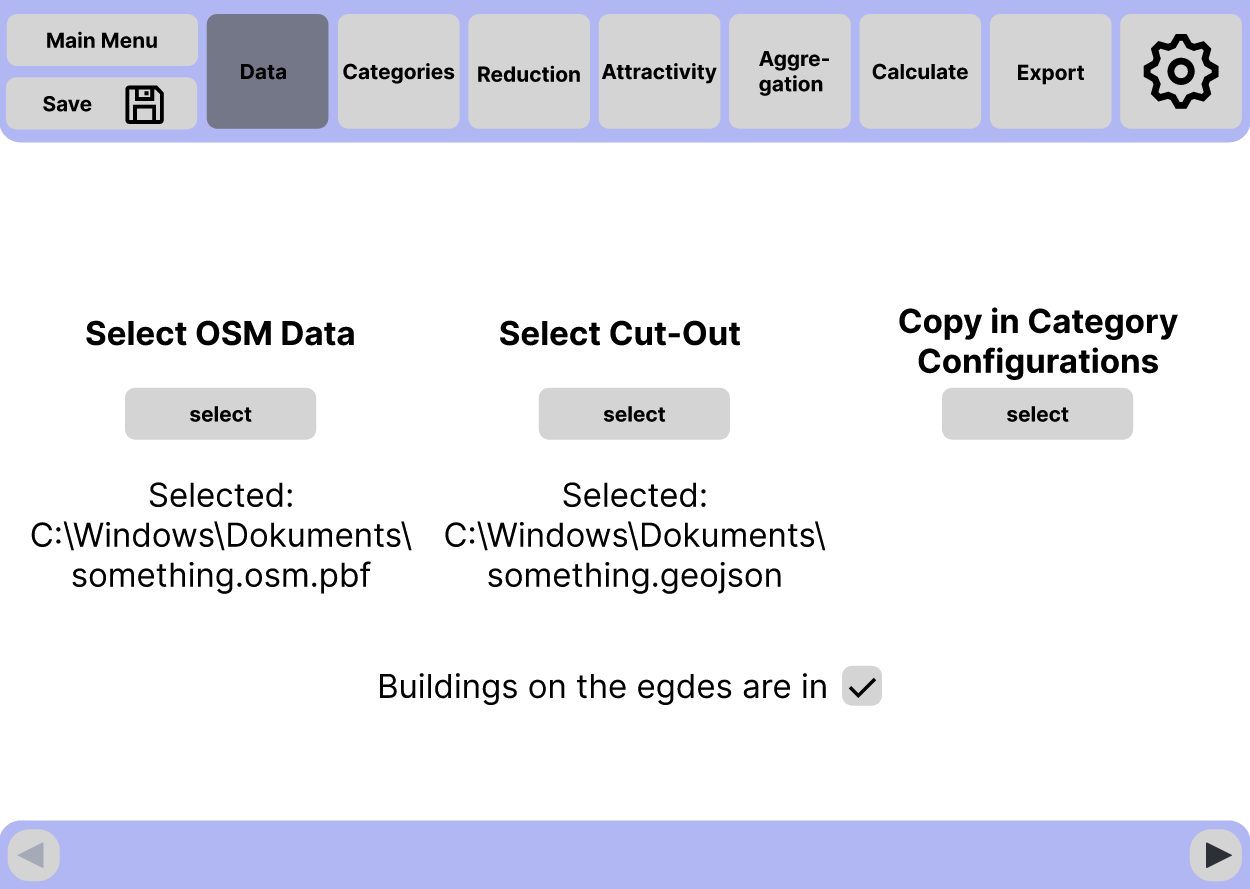
\includegraphics[width=1\textwidth]{pictures/Data.png}
    \caption{Data}
\end{figure}

\begin{figure}
    \centering
    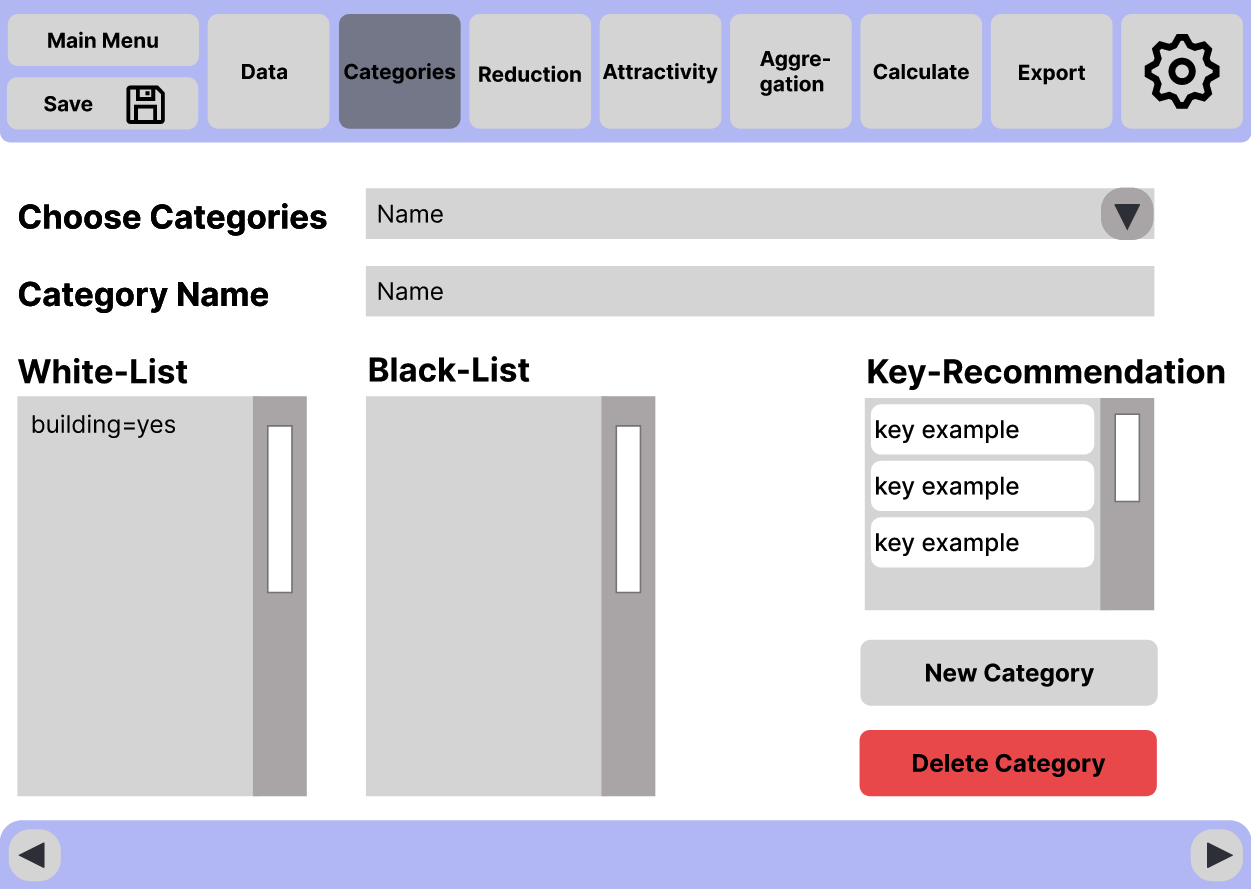
\includegraphics[width=1\textwidth]{pictures/Categories.png}
    \caption{Categories}
\end{figure}

\begin{figure}
    \centering
    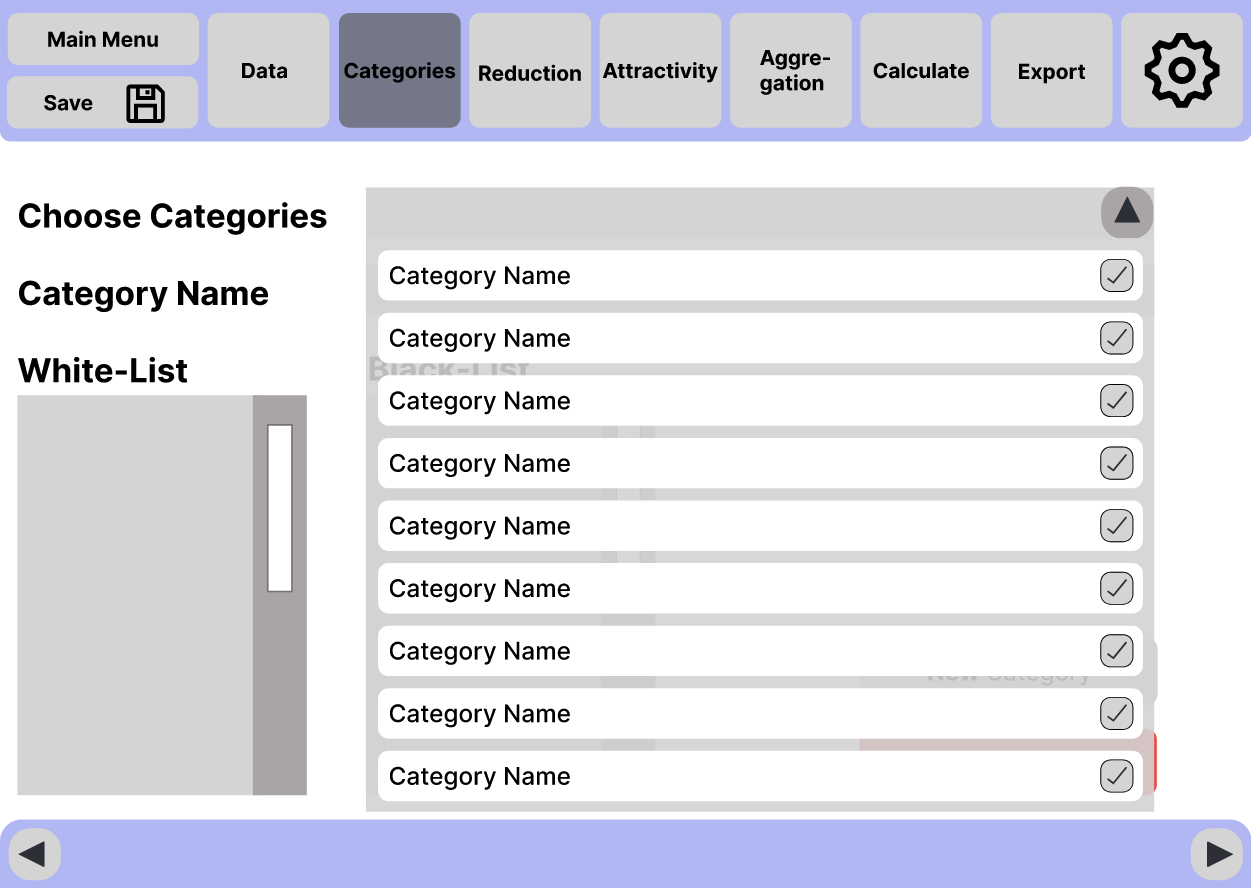
\includegraphics[width=1\textwidth]{pictures/Categories 2.png}
    \caption{MCategories 2}
\end{figure}

\begin{figure}
    \centering
    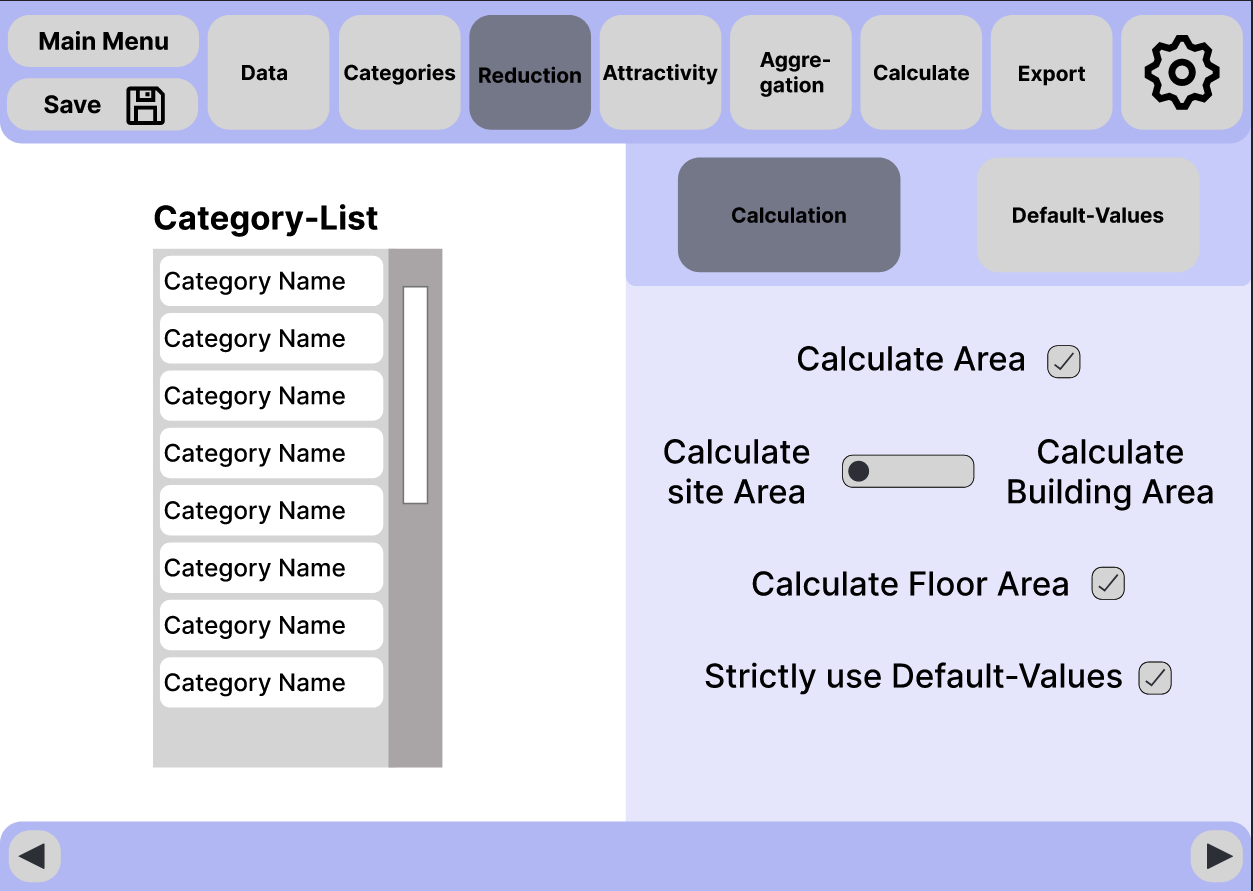
\includegraphics[width=1\textwidth]{pictures/Reduction.png}
    \caption{Reduction}
\end{figure}

\begin{figure}
    \centering
    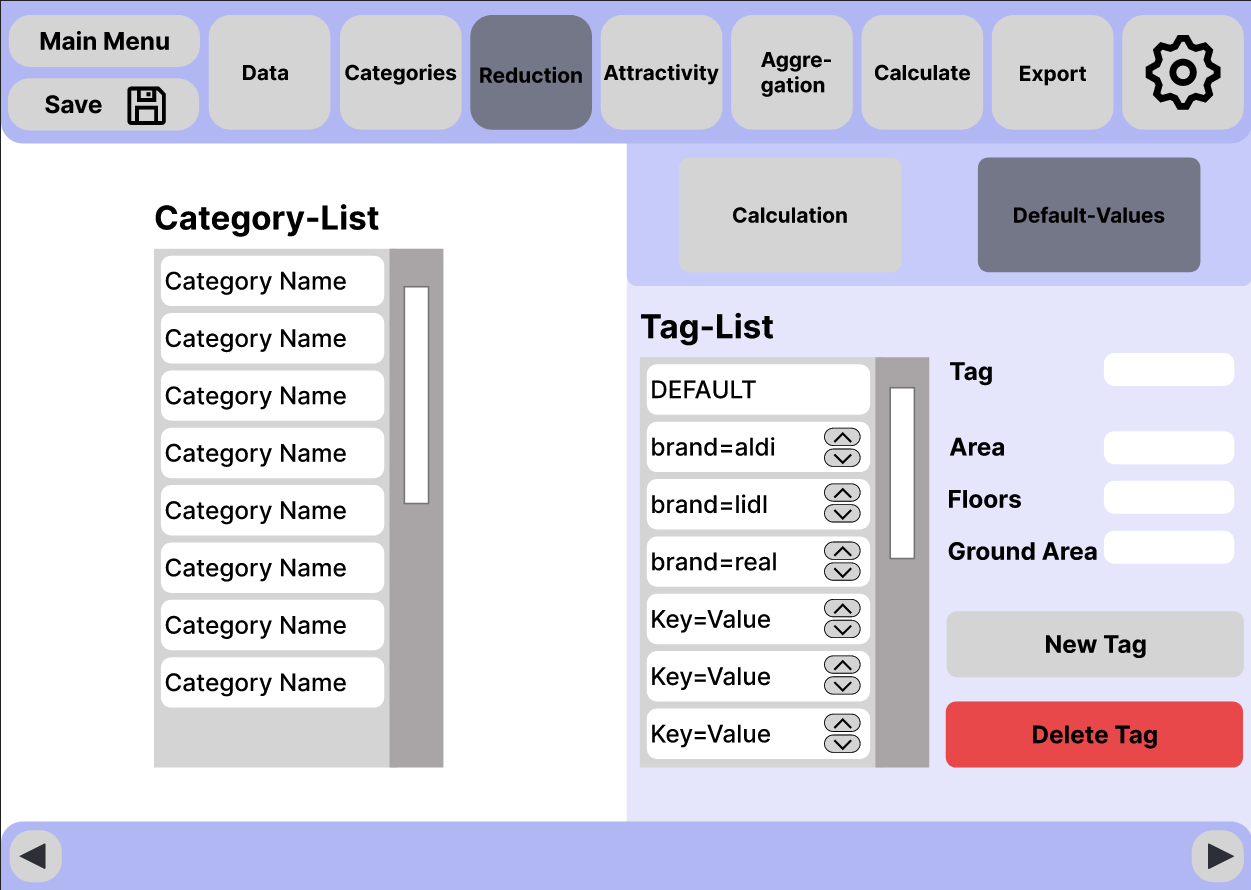
\includegraphics[width=1\textwidth]{pictures/Reduction 2.png}
    \caption{MReduction 2}
\end{figure}

\begin{figure}
    \centering
    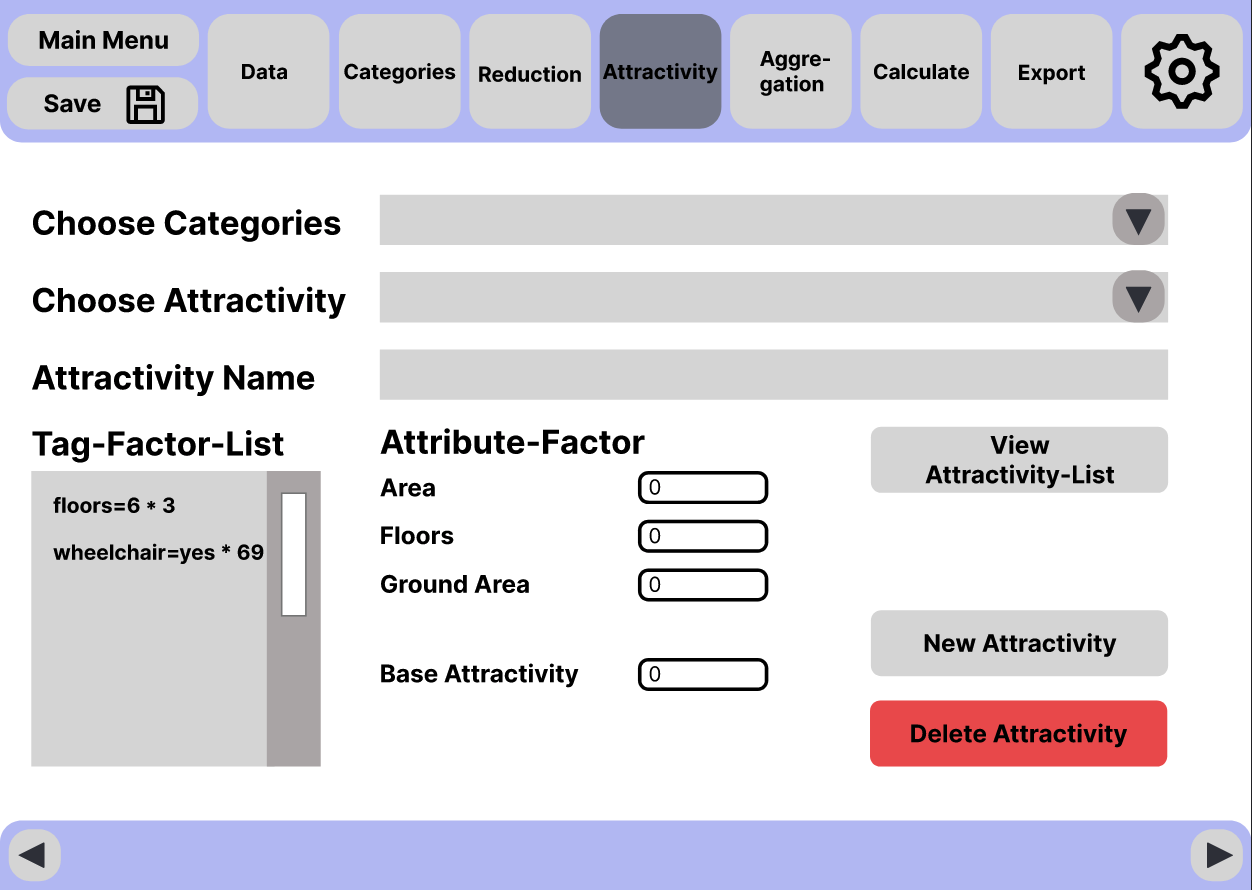
\includegraphics[width=1\textwidth]{pictures/Attractivity.png}
    \caption{Attractivity}
\end{figure}

\begin{figure}
    \centering
    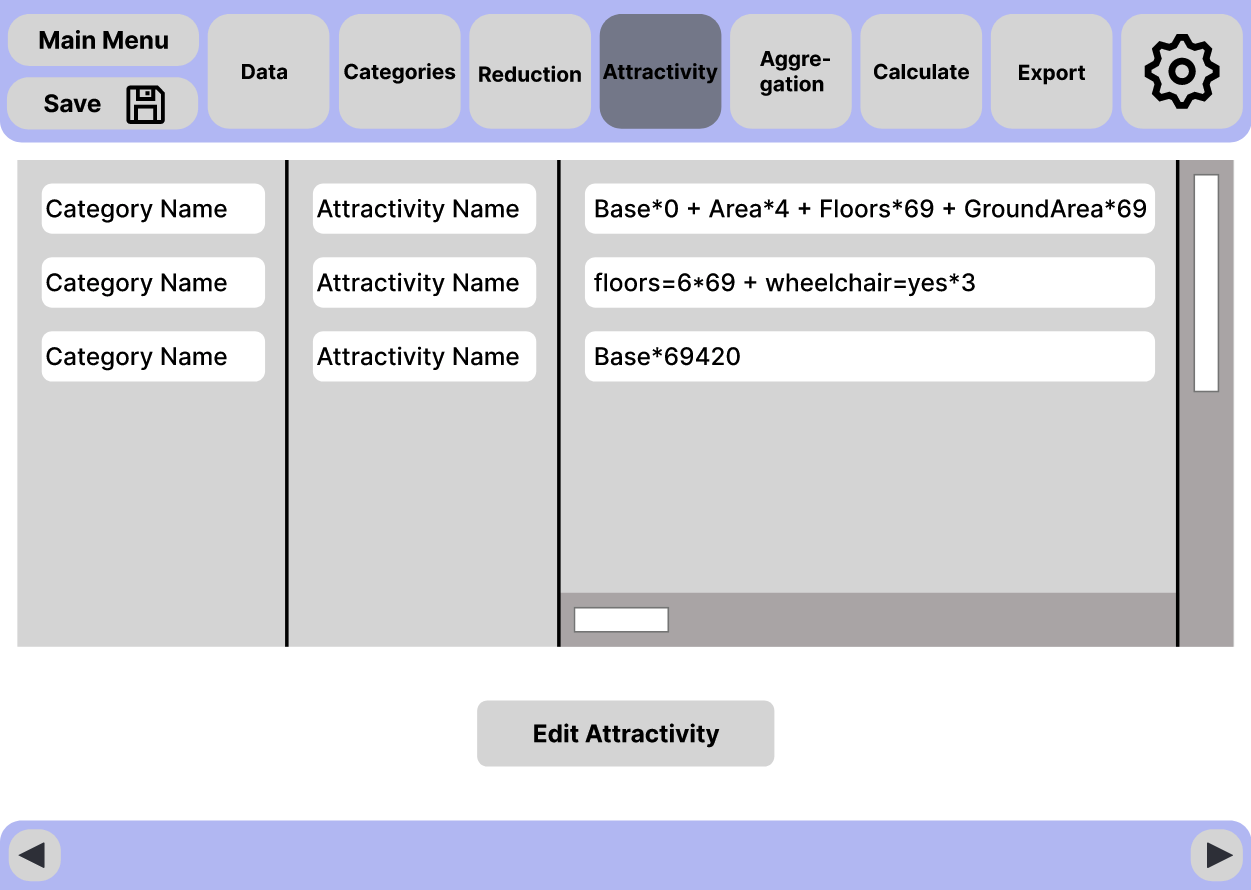
\includegraphics[width=1\textwidth]{pictures/Attractivity 2.png}
    \caption{Attractivity 2}
\end{figure}

\begin{figure}
    \centering
    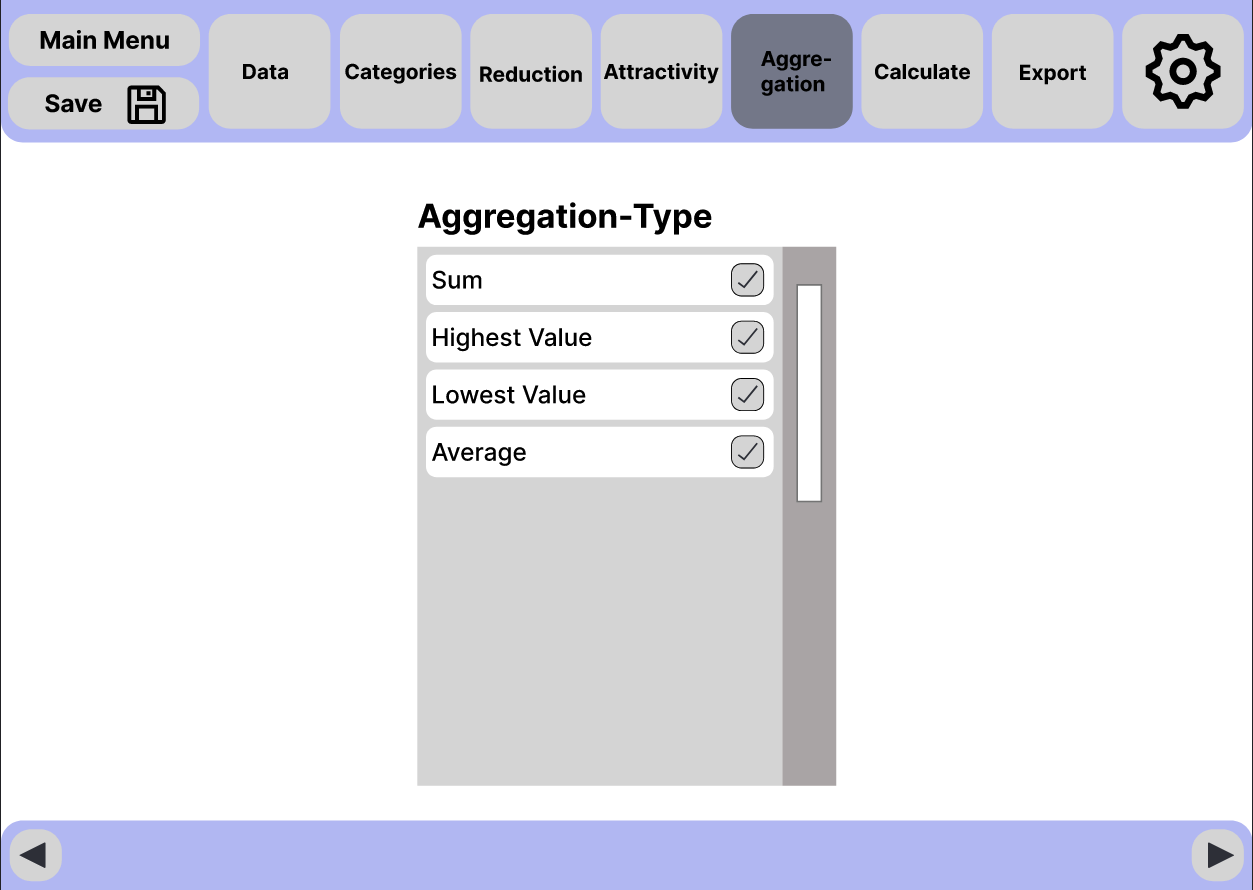
\includegraphics[width=1\textwidth]{pictures/Aggregation.png}
    \caption{Aggregation}
\end{figure}

\begin{figure}
    \centering
    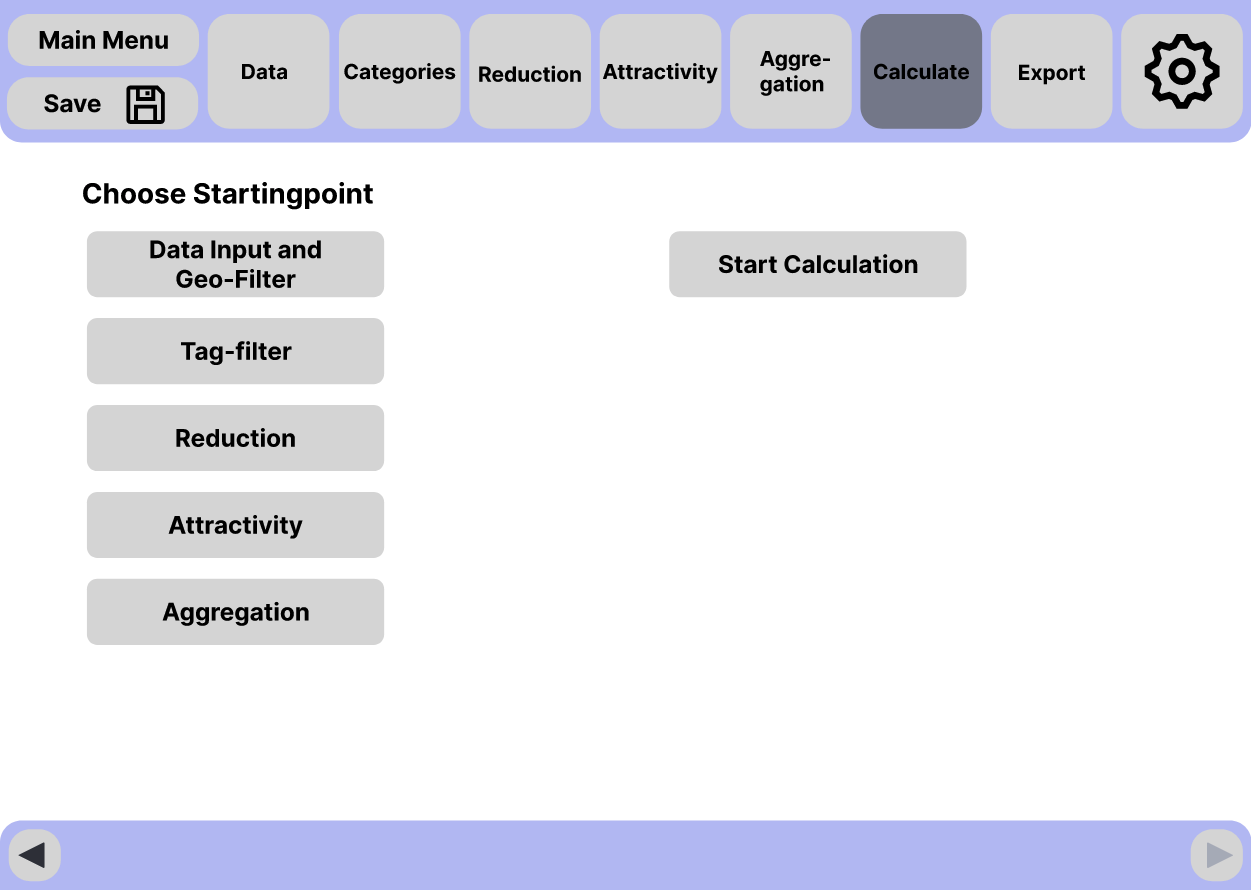
\includegraphics[width=1\textwidth]{pictures/Calculate.png}
    \caption{Calculate}
\end{figure}

\begin{figure}
    \centering
    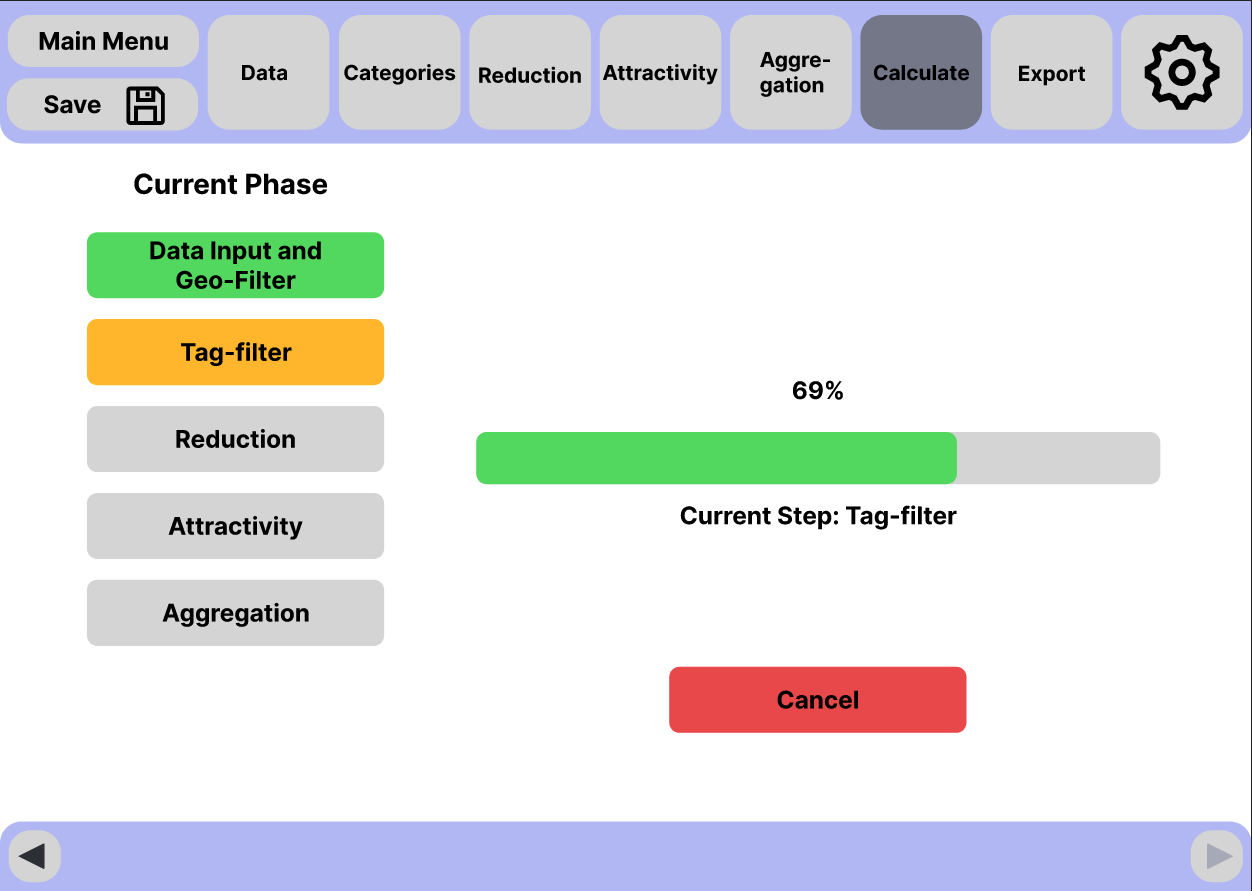
\includegraphics[width=1\textwidth]{pictures/Calculate 2.png}
    \caption{Calculate 2}
\end{figure}

\begin{figure}
    \centering
    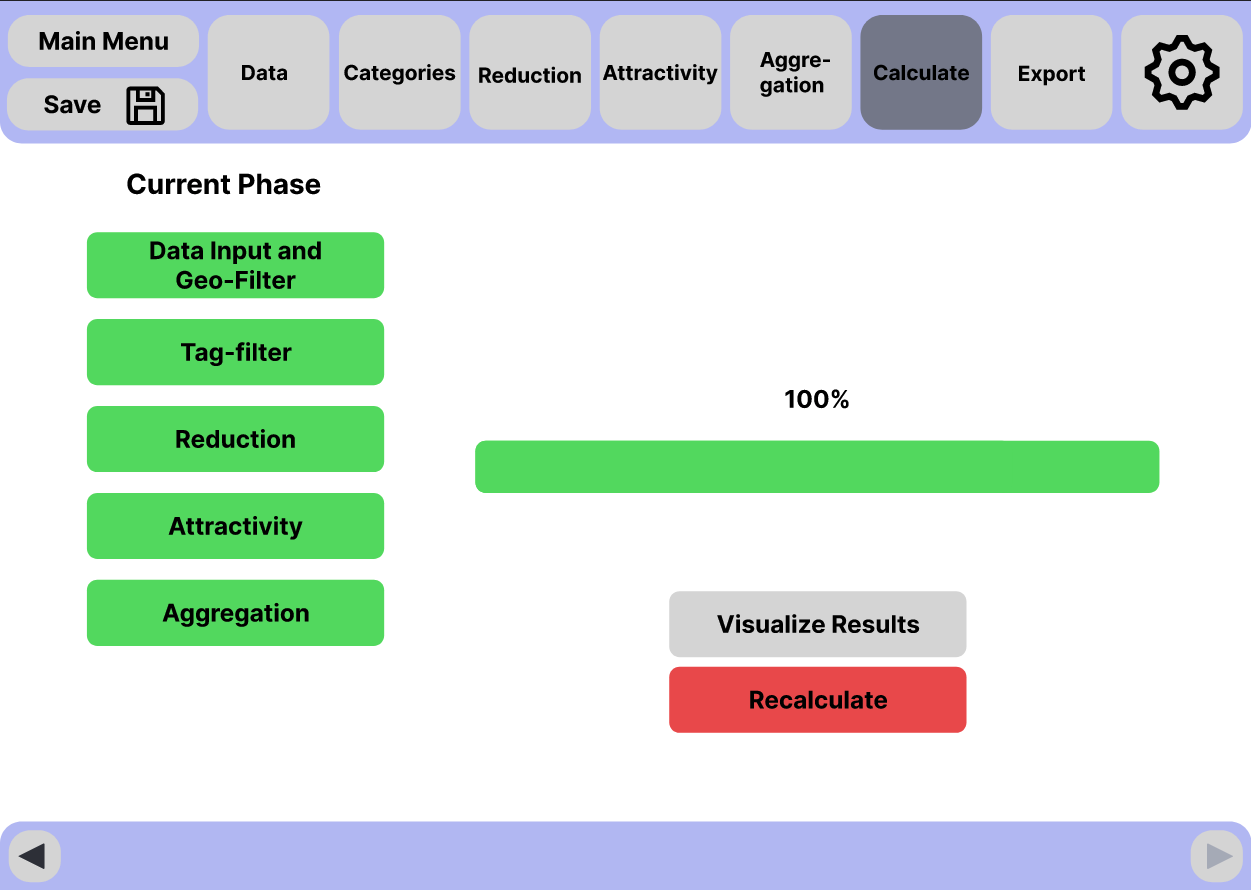
\includegraphics[width=1\textwidth]{pictures/Calculate 3.png}
    \caption{Calculate 3}
\end{figure}

\begin{figure}
    \centering
    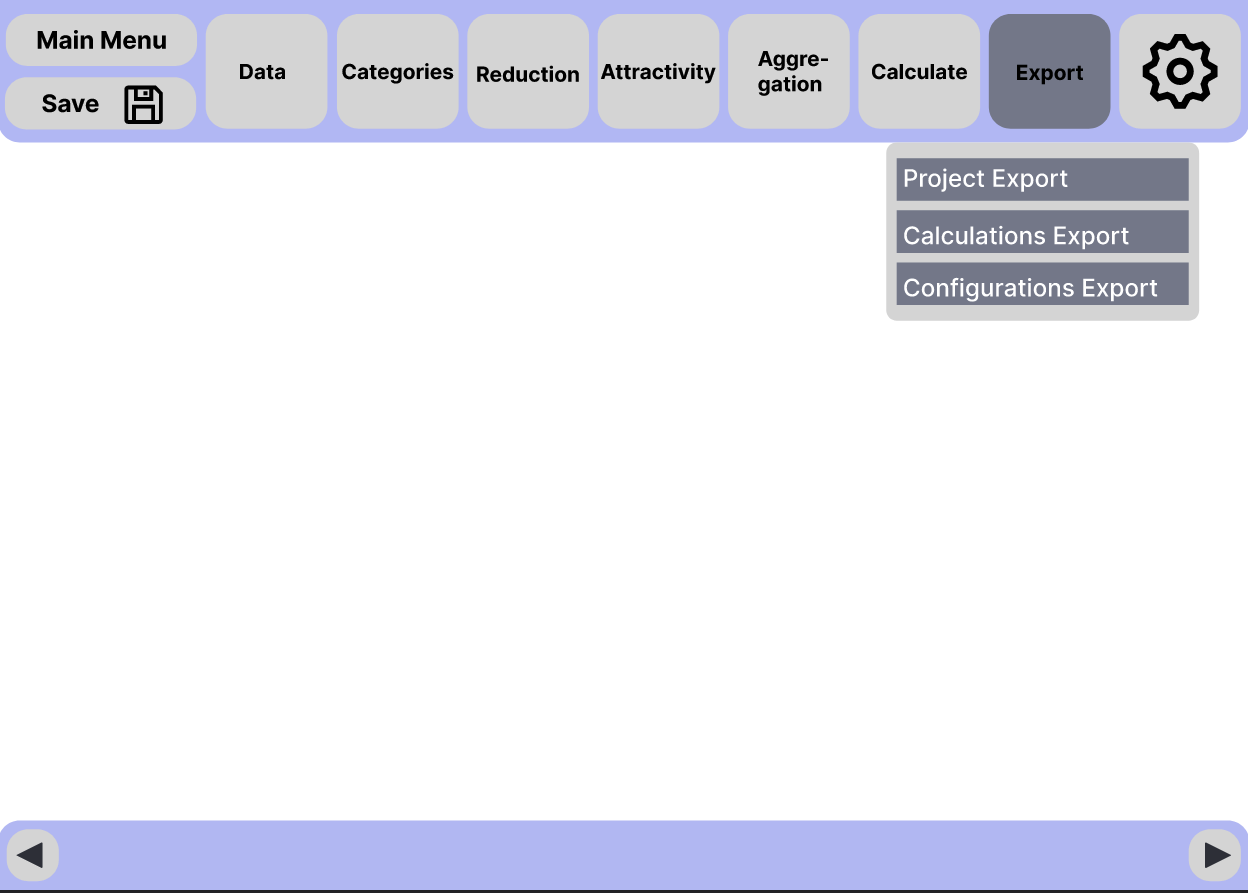
\includegraphics[width=1\textwidth]{pictures/Export.png}
    \caption{Export}
\end{figure}

\begin{figure}
    \centering
    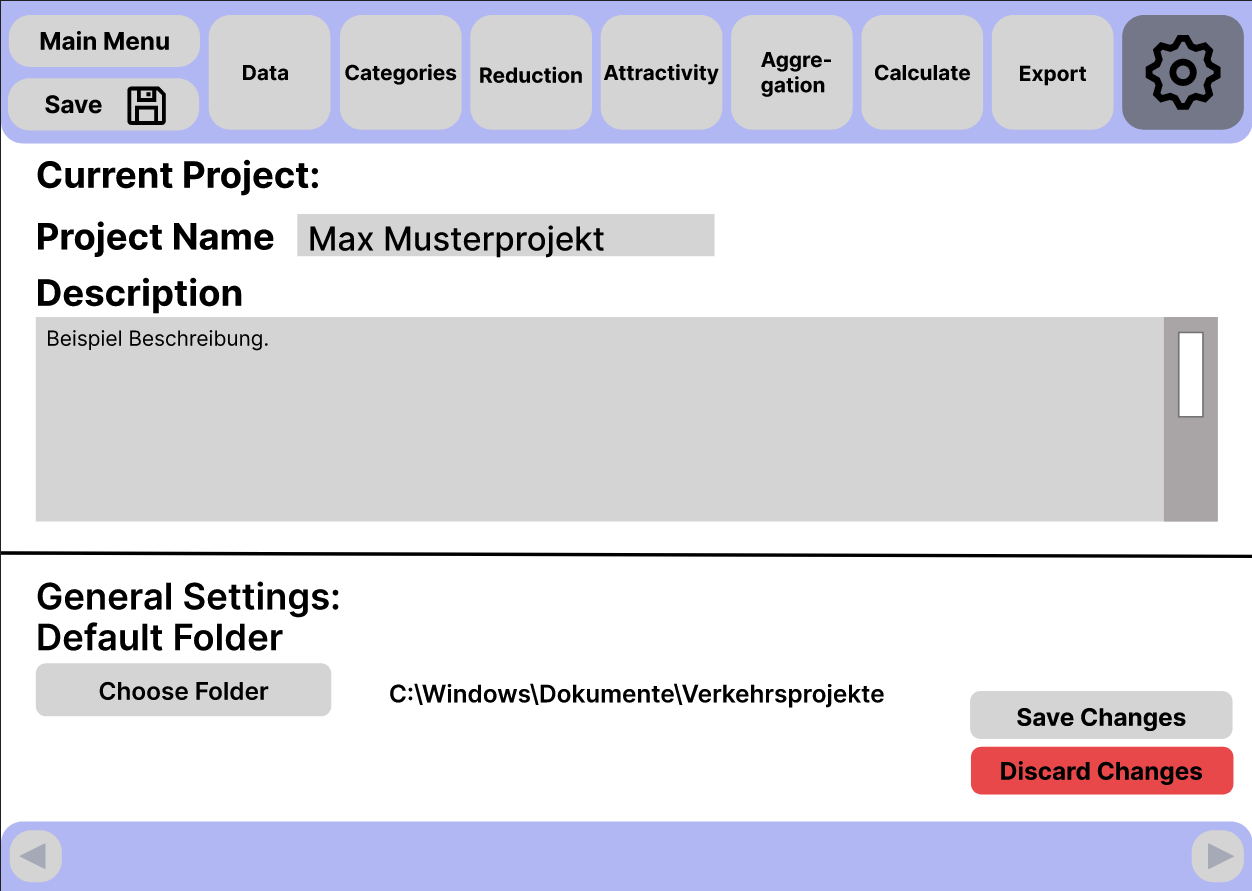
\includegraphics[width=1\textwidth]{pictures/Options.png}
    \caption{Options}
\end{figure}

\newpage

\begin{figure}
    \centering
    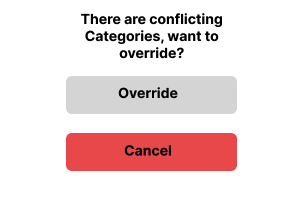
\includegraphics[width=1\textwidth]{pictures/Conflict PopUp.png}
    \caption{Conflict PopUp}
\end{figure}

\begin{figure}
    \centering
    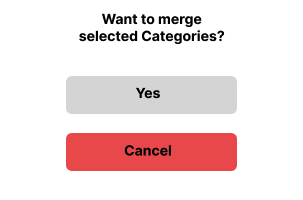
\includegraphics[width=1\textwidth]{pictures/Merge PopUp.png}
    \caption{Merge PopUp}
\end{figure}

\begin{figure}
    \centering
    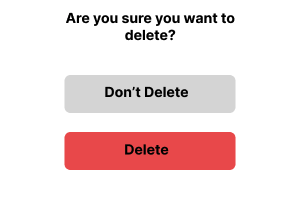
\includegraphics[width=1\textwidth]{pictures/Delete PopUp.png}
    \caption{Delete PopUp}
\end{figure}

\begin{figure}
    \centering
    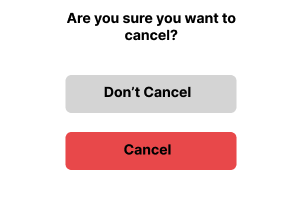
\includegraphics[width=1\textwidth]{pictures/Cancel PopUp.png}
    \caption{Cancel PopUp}
\end{figure}

\begin{figure}
    \centering
    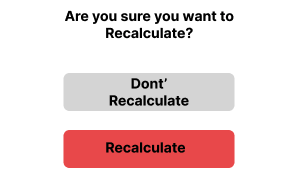
\includegraphics[width=1\textwidth]{pictures/Recalculate PopUp.png}
    \caption{Recalculate PopUp}
\end{figure}

\newpage



\section{Technische Produktumgebung}
In diesem Kapitel wird die technische Umgebung des Produktes beschrieben.

\subsection{Software}
\begin{itemize}
    \item Implementierungssprache der Anwendung: Python
    \item Betriebssystem: Windows 10/11
\end{itemize}

\subsection{Hardware}
\begin{itemize}
    \item Laptop mit 8 GB RAM und i5 4 Kerne (8 log.) für kleine Instanzen.
    \item Workstation mit 125 – 250 GB RAM und 8–16 Kerne für große Instanzen.
\end{itemize}

\subsection{Produktschnittstellen}
Die Anwendung bietet eine Benutzerschnittstelle über ein GUI zur Verfügung.
\newpage





\section{Glossar}

\textbf{Aggregation}\\
Verfahren zum Zusammenfassen mehrerer Attraktivitätsattribute innerhalb einer Verkehrszelle.

\textbf{Attribut}\\
Eigenschaft eines OSM-Elements. Wird aus den OSM-Tags des OSM-Elements während der Punktreduktion berechnet.


\textbf{Attraktivitätsattribut}\\
Eigenschaft eines geografischen Objektes. Beschreibt die Attraktivität eines Ortes bezüglich einer bestimmten Tätigkeit. Wird aus Attributen berechnet.

\textbf{Checkbox}\\
Kästchen, die eine binäre Beziehung darstellen. Wird ein Kästchen markiert, wird die zugehörige Option ausgewählt.

\textbf{Default-Values}\\
Vordefinierte Standardwerte, die zu einer Berechnung herangezogen werden können.

\textbf{Dropdown-Menü}\\
Verbirgt sich hinter einem einzelnen Knopf. Wird das Dropdown-Menü über diesen Button geöffnet, erscheinen mehrere Buttons, die zur weiteren Steuerung verwendet werden können.

\textbf{Explorer}\\
Auflistung aller Ordner, die sich im Computerspeicher befinden. Hier kann der Speicherpfad ausgewählt werden.

\textbf{Kategorie}\\
Einheit zum Organisieren von OSM-Elementen. Eine Kategorie definiert eine Menge an OSM-Elementen und weißt dieser Eigenschaften zu.

\textbf{Standardkategorien}\\
Kategorien, die standardmäßig in jedem Projekt vorhanden sind.

\textbf{Node}\\
Objekt in OSM.

\textbf{OSM}\\
Abkürzung für OpenStreetMap. OpenStreetMap ist ein freies Projekt, das Geodaten sammelt, strukturiert und für die freie Nutzung in einer Datenbank bereitstellt.

\textbf{OSM-Objekt}\\
Eintrag in der OSM-Datenbank. Ist definiert durch seine Tags.

\textbf{OSM-Datei}\\
Datei, die OSM-Objekte enthält.

\textbf{Punktreduktion}\\
Verfahren zur Abbildung von Gebäuden auf Punkte. Dabei werden den Punkten Attribute zugewiesen.

\textbf{Repository}\\
Zentrale Ablage, in der digitale Daten, Dokumente, Objekte und Programme mit ihren Metadaten verwaltet werden.

\textbf{Tag}\\
Eigenschaft eines OSM-Objekts. Bestehend aus einem 'key' und einer 'value'.

\textbf{Tag Filter}\\
Die Gruppierung von OSM-Elementen anhand ihrer Tags.

\textbf{Verkehrsnachfragemodell}\\
Ein Verkehrsnachfragemodell ist ein Modell, das alle relevanten Entscheidungsprozesse der Menschen nachbildet, die zu Ortsveränderungen führen. Im Personenverkehr umfassen diese Entscheidungen die Aktivitätenwahl, die Zielwahl, die Verkehrsmittelwahl, die Abfahrtszeitwahl und die Routenwahl.

\textbf{Verkehrszelle}\\
Bezeichnet einen räumlich abgegrenzten Teil eines Untersuchungsgebietes, der als Bezugseinheit bei der Verkehrsanalyse und Verkehrsprognose dient.

\textbf{Untersuchungsgebiet}\\
Räumliches Gebiet, das von der Anwendung untersucht wird. Disjunkte Vereinigung der Verkehrszellen. Wird durch den räumlichen Filter definiert.

\textbf{Aggregations-Vefahren}\\
Abbildung einer Menge von Attraktivitätsattributen auf einen numerischen Wert. Beispiele sind die Summe, das Produkt oder das arithmetische Mittel.

\textbf{Geofilter}\\
Verfahren zum Definieren der Zugehörigkeiten von OSM-Objekten zu einem geografischen Gebiet.

\textbf{Räumlicher Filter}\\
Methode zur genaueren Definition eines Geofilters. Entscheidet ob OSM-Elemente die sich nur teilweise in einem Gebiet befinden, diesem zugehörig sind.

\textbf{Projekt}\\
Organisationseinheit. Gesamtheit von zusammengehörenden Konfigurationen.

\textbf{Projektordner}\\
Verzeichnis. Organisiert alle Konfigurationsdateien eines Projektes.

\textbf{Projektstandardordner}\\
Verzeichnis, in welchem standardmäßig Projekte gespeichert und geladen werden.

\textbf{Berechnungsphase}\\
Zeitlich zusammenhängender Abschnitt des Berechnungsvorgangs. Es gibt die Phasen OSM-Daten, räumlicher Filter, Tag Filter, Punktreduktion, Attraktivitätsberechnung und Aggregation.

\textbf{Konfigurationsphase}\\
Abschnitt der Konfiguration eines Projektes

\textbf{Seite}\\
Ein inhaltlich zusammenhängender Abschnitt der GUI, welcher gleichzeitig angezeigt wird.



\end{document}